\documentclass[a4paper,11pt]{report}
\usepackage[]{amsmath}
\usepackage[]{physics} % \bra, \ket etc
\usepackage{graphicx} %Pour les figures je crois
\usepackage{hyperref}
\usepackage[
    backend=biber, 
    natbib=true,
    style=numeric-comp,
    sorting=none, %Pour faire apparaitre les refs dans l'ordre
    hyperref=true
]{biblatex} %Imports biblatex package
\addbibresource{Bib_ch1.bib} %Import the bibliography file

\usepackage{amssymb} %quelques symboles dont gtrsim /lesssim
\usepackage{subcaption} % package pour faire des subfigures
\usepackage{multirow} % package pour multirow/multicolumn
\usepackage{booktabs} % package pour top/mid/bottom rule
\usepackage{tcolorbox} % toujours plus de boites
\usepackage{xcolor} % Pour avoir des couleurs dans les équations

\DeclareUnicodeCharacter{0308}{HERE!HERE!} % je vais pas m'énerver, mais un peu quand meme

\title{}
\begin{document}
\chapter{Introduction to Nitrogen-Vacancy centers and their common usage}
The aim of this first chapter is to introduce concepts related to Nitrogen-vacancy (NV) centers, to the diamond material, and to the dipole-dipole interaction which are necessary to explain the work presented in the later chapters.

In this introductory chapter, we will first cover the material aspects of NV centers by focusing on the creation process of synthetic diamonds and the required steps to create NV defects inside them. We will then cover the fundamentals of NV physics, including the NV center optical and spin properties, basic experiments with NV centers and the various relaxations times ($T_1$,$T_2$,$T_2^*$) which characterizes the NV center's spin. Finally we will present the dipole-dipole interaction between two spins and the concept of cross-relaxation.

\section{The NV center as a physical object}
\begin{figure}[h!]
\centering
\includegraphics[width=0.9\textwidth]{Figures/diamant_et_NV}
\caption{From the diamond to the NV center. a) Drawing of a bulk diamond. We consider a diamond to be ``bulk" if it is bigger than a few 100 $\mu$m. b) Drawing representing a fluorescence microscopy image of a diamond surface. The red fluorescent spots symbolize NV centers photoluminescence. c) Zoom-in on the crystalline structure of an NV center. Black balls represent carbon atoms}
\label{diamond+NV}
\end{figure}
The NV center is a particular defect in diamond. Before studying the NV centers properties, we must first discuss the diamond itself and answer these questions: How are diamond created, what kind of defects are there in diamond, and how to specifically create NV defects. The field of material science related to diamonds and NV centers is a rich and complex one, and this section will only introduce basic notions regarding these subjects.

Fig. \ref{diamond+NV} illustrates the various scales to consider in the study of NV centers. Starting with a bulk diamond, typically few mm wide, then zooming-in on the diamond surface with an optical microscope to find fluorescent spots corresponding to the photoluminescence of NV centers. Standard confocal microscopy is limited in its resolution to the $\sim \mu$m range, but if it was possible to zoom-in even further, we would see the atomic structure of a few \AA \ illustrated in the last panel. 
\subsection{Diamond material overview}
\begin{figure}[h!]
\centering
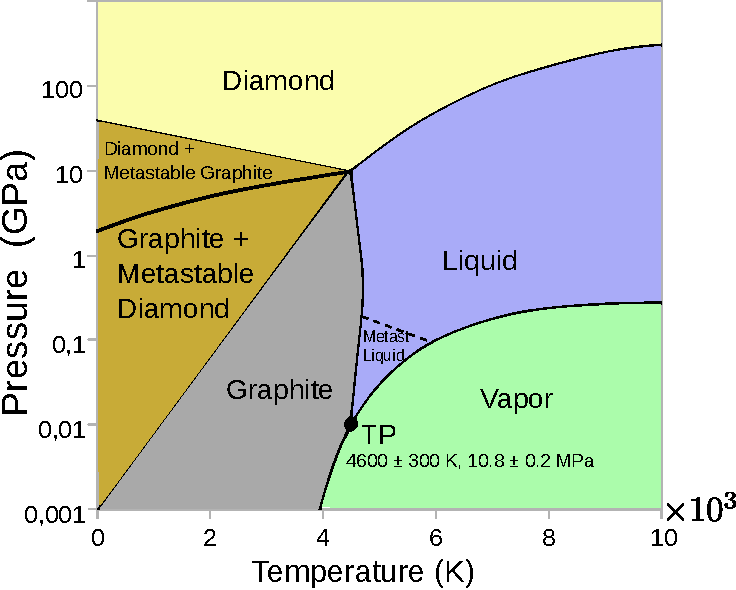
\includegraphics[width=0.6\textwidth]{Figures/phase_diagram_carbon_wiki}
\caption{Pressure-temperature phase diagram of elemental carbon. Credits: Wikimedia commons, adapted from \citep{bundy1989pressure, bundy1996pressure}.}
\label{carbon phase diagram}
\end{figure}

Diamond is a remarkable material in many aspects, it is famous for having the highest hardness and thermal conductivity of any natural material, and for its high optical refractive index and optical dispersion which makes it an extremely valuable crystal in jewelry.

Diamond is also famous for being extremely rare in nature, even though its only constituent, carbon, is one of the most abundant element on the Earth surface. The reason being that graphite, and not diamond, is the thermodynamically stable phase of carbon under ambient conditions.

Fig. \ref{carbon phase diagram} shows the PT phase diagram of elemental carbon. We can see that diamond becomes the thermodynamically stable phase only for pressure above a few GPa, $10^4$ times higher than atmospheric pressure. Even though diamond is unstable under ambient conditions, the extremely high energy activation needed to break the sp$^3$ bond between two carbon atoms means that the kinematics of the $C_{\rm diamond} \to C_{\rm graphite}$ transition is almost completely frozen. In many ways diamonds are more stable than graphite under ambient condition due to their relative chemical inertness.

Where the thermodynamic equilibrium really matters is for the crystallization process. The higher pressure needed to reach the diamond-stable region can only be found naturally deep under the earth crust, typically between 150 and 240 km below sea level \citep{tappert2011diamonds}, which explain their rarity. It also explains why, despite many previous attempts, diamonds were only synthetically produced in 1953 \citep{barnard2000diamond}, more than 50 years after the first synthetic sapphires. To this day, artificial diamond synthesis remains an active field of research \citep{shenderova2019synthesis, achard2020chemical}.

Diamonds, either natural or artificial, are used in the lab and in industry for their extreme sturdiness, with applications ranging from abrasive to diamond anvil cells \citep{jayaraman1983diamond}. More recently, diamonds have been the object of optics and electronics applications. For both of these fields however, the focus is no longer solely on the diamond but also on the defects hosted inside it.

\subsection{Point defects in diamond}
\begin{figure}[h!]
\centering
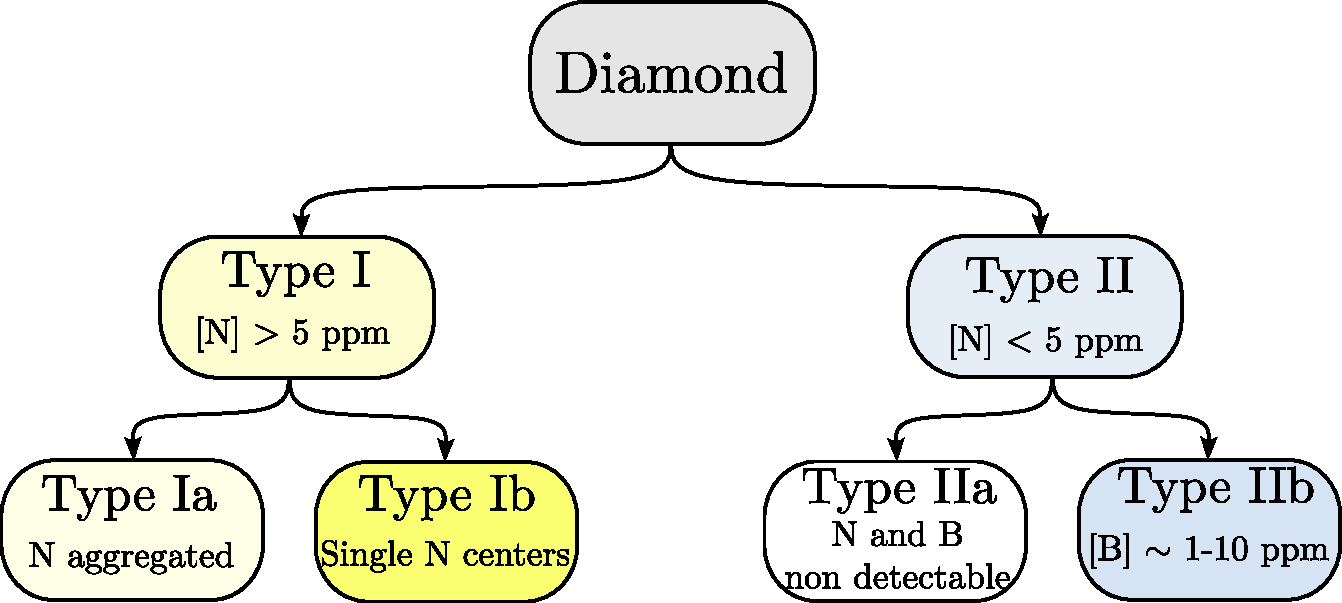
\includegraphics[width=0.9\textwidth]{Figures/Diamond_type}
\caption{Traditional classification of diamonds, based on \citep{tappert2011diamonds}}
\label{diamond type}
\end{figure}
Diamond in its intrinsic form is an insulator with a bandgap of $\sim 5.47\ \rm eV$ and is transparent from far infrared to deep UV. As any crystal however, diamond is prone to defects. We will focus here on point-like (0D) defects and omit structural defects such as dislocations, even though those too can affect the optical properties of the diamond \citep{collins2000colour}. 

Point-like defects can be constituted by the absence of a carbon atom (``vacancies"), an interstitial defect between two carbon atoms or the substitution of a carbon atom with another atom. These impurities result in unpaired electron or holes localized around the impurity site. This localization causes discrete energy levels for the holes or the electrons, some of which lie inside the diamond bandgap and impact the crystal optical and electrical properties. 

Defects with electronic transitions in the optical range are called ``colored centers" as they are responsible for the coloring of the gems.  Over 20 elements are known to form colored centers when introduced in diamond \citep{zaitsev2013optical, shenderova2019synthesis}, and each of these elemental atoms can form several defects. Nitrogen alone can form more than 50 different colored centers \citep{dobrinets2016hpht, ashfold2020nitrogen}.

Nitrogen, and to a lesser extant boron, are the most commonly found extrinsic elements in natural diamond. The traditional classification of diamond is presented in Fig. \ref{diamond type}. It is based on the N and B concentration, with a threshold of a few ppm (part per million) for each species as this was the smaller amount easily detectable through IR absorption. Type Ia diamonds contain clustered N defects such as the B-center (N$_4$V defect). In contrast, type Ib diamond mostly contains C-center which are single substitutional N$_s$ defects, also referred to as P1 centers in the spin community. Type IIb diamond contains boron impurities which give them a blueish-grey color, and type IIa diamond contains no detectable impurities via IR absorption \citep{ashfold2020nitrogen}.

Nitrogen-vacancy centers are a rare occurrence in both natural diamonds and untreated synthetic diamonds, but we will see later that the much more common N$_s$ defects can be converted in NV centers. When working with NV centers, the starting crystal is therefore often a type Ib diamond if one wants to work with ensemble, or a type IIa diamond if one wants to work with single NV centers \footnote{In order to isolate single NV in a confocal optical spot, the concentration needs to be [NV] $<$ 1 ppb.}.

The boron defects are mainly studied in the context of p-doped diamond semi-conductor: a concentration of [B] $\approx 1000\ \rm ppm$ is needed to achieve a significant overlap between the impurity sites, which turns the diamond into a semi-metal \citep{macpherson2015practical}. Other defects of interest, generally not present naturally but introduced voluntarily, include P and S defects to create n-doped diamond \citep{das2022diamond} (still an active field of research), as well as group IV-vacancy defects (SiV, GeV, SnV, PbV) for quantum optics application \citep{bradac2019quantum}. 

The NV center however remains by far the most studied defect in diamond due to its unique spin properties which will be detailed below.

\subsection{Creation of synthetic diamond for optics and electronics applications}
\begin{figure}[h!]
\centering
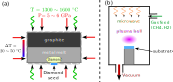
\includegraphics[width=\textwidth]{Figures/HPHT_and_CVD}
\caption{Schematics of HPHT (a) and CVD (b) growth process as detailed in main text}
\label{HPHT and CVD}
\end{figure}

Almost all diamonds used in optics or electronics experiments today are synthetic, due to the higher control of the growth process required for these applications. There are two main competing technologies for the growth of large ($\mu \rm{m} \sim \rm{mm}$) single crystal diamonds: High pressure high temperature growth (HPHT) and chemical vapor deposition growth (CVD). Both of these processes have their own specificities which are detailed below.

\subsubsection{HPHT growth}

HPHT was the first commercially viable process for synthetic diamonds, starting from the 1950s \citep{barnard2000diamond, bundy1955man}. The basic idea of HPHT synthesis is to reconstruct an environment where diamond is the thermodynamically stable phase of carbon, similarly to the growth process of natural diamond below the earth surface. 

Fig. \ref{HPHT and CVD}-a) illustrates the apparatus of HPHT synthesis: a carbon source (graphite) and a solvent metal composed of transition metals (Fe, NI, Co typically \citep{bundy1963direct}) are put under $5 \sim 6$ GPa pressure in a press and heated to temperatures $\geq 1300\ ^\circ$C. A diamond crystal seed is put in the metal melt and a temperature gradient insures that the carbon migrates from the graphite to the diamond.

The first synthesis of HPHT diamonds were all of type Ib due to unwanted nitrogen pollution in the metal melt. The first HPHT type IIa diamonds were produced in the late 90s by adding other elements to the metal bath (Ti, Al, Zr) which would react preferentially with nitrogen and prevent its incorporation in the diamond \citep{burns1999growth, sumiya2002growth}.

\subsubsection{CVD growth}

Diamond growth by CVD also started in the 50s, but the first reasonable growth rates were only achieved in the 80s \citep{matsumoto1982growth, matsumoto1982vapor, kamo1983diamond}. Unlike HPHT, CVD operates in a regime where diamond is not the thermodynamically stable phase. It relies therefore heavily on catalysts to stabilize the diamond phase versus the graphite one. 

The main catalyst used is atomic hydrogen because it etches the $C-C$ sp$^2$ bonds (graphite) faster than it does sp$^3$ bonds (diamond) \citep{gracio2010diamond}. In modern CVD growth, hydrogen is by far the most abundant element in the gas phase: the precursor gases used for the growth are typically CH$_4$ and H$_2$ in proportions of $1-5\%$ and $95-99\%$ respectively \citep{achard2020chemical}.

Fig. \ref{HPHT and CVD}-b) illustrates the apparatus of a microwave plasma reactor: it consists in a modified vacuum chamber which acts as a microwave resonator. The microwave creates a plasma ball from the the precursor gases with a temperature $T_{\rm plasma} \geq 3000 ^\circ$C \citep{ashfold2020nitrogen}, enough to dissociate the $H_2$ gas in atomic hydrogen \citep{balmer2009chemical}. The plasma acts as the carbon source for the diamond growing on top of the substrate, and as the catalyst to favor the diamond phase. The substrate is kept at a temperature $700 \sim 1100\ ^\circ$C during the growth.

Other sources can be used to create the high temperature required for atomic hydrogen, such as a tungsten hot filament \citep{haubner1993diamond}, electrical discharge (arcjet) \citep{luque1998excited} or even an oxygen-acetylene combustion flame \citep{bachmann1991towards}.

If the CVD reactor is well made, the main sources of extrinsic impurities in the diamond comes from the source gasses \citep{balmer2009chemical}. The commercial availability of source gases containing less than $\sim$ ppm impurities made possible the growth of  high purity type IIa CVD diamonds \citep{kasu2003high, twitchen2004high, tallaire2006characterisation}.

\medskip
Both HPHT and CVD processes can produce diamonds of high quality for quantum optics or electronics application, each with their own pros and cons. HPHT offers better scalability for thick crystals ($\sim \rm mm$) and allows the incorporation of heavy atoms (Ge \citep{palyanov2015germanium} , Sn \citep{ekimov2019effect}) which can be hard to incorporate from a gas phase. CVD on the other hand allows more versatility in the control of the impurities introduced in the crystal, including an isotopic control on both the impurities and the carbon itself. A particular advantage of CVD growth is the possibility of $\delta$-doping where a specific defect is grown only within a thin layer of the crystal, as low as 5 nm \citep{ohno2012engineering, ishikawa2012optical, ohashi2013negatively}.

\subsection{Optimizing NV center formation}
\begin{figure}[h!]
\centering
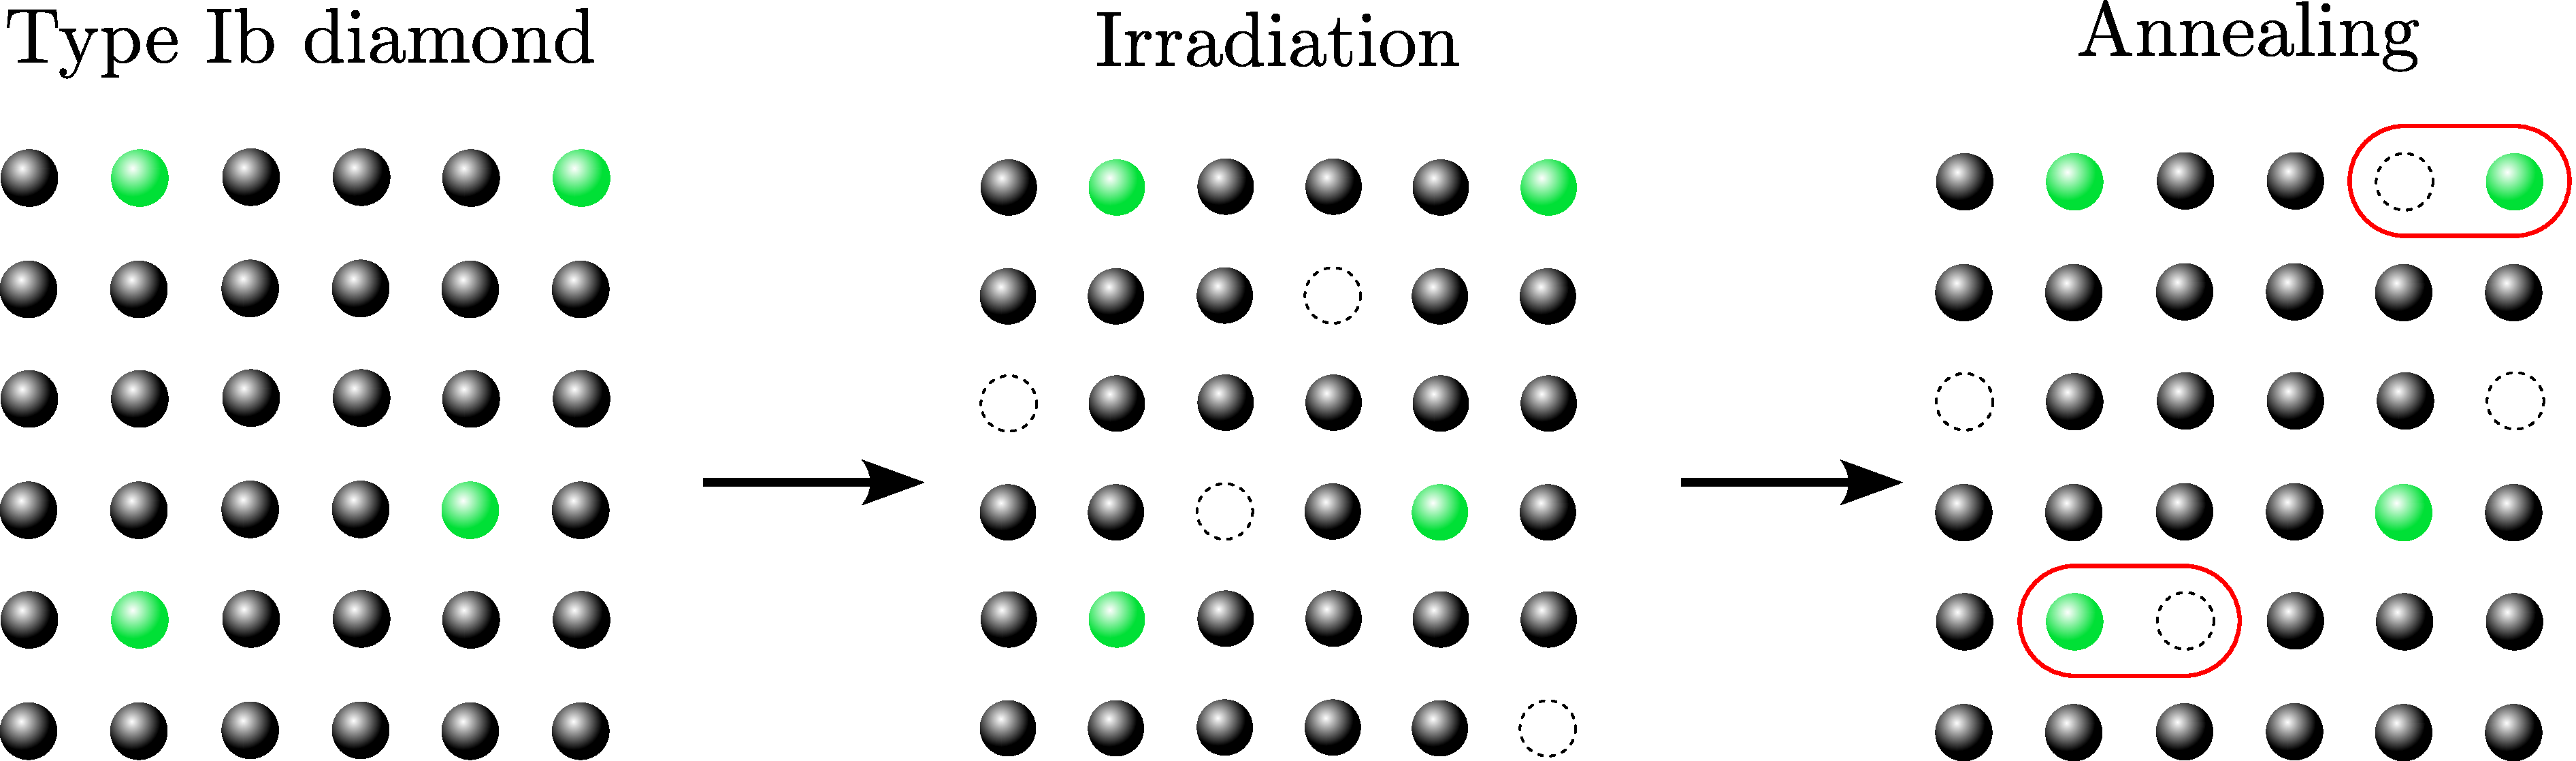
\includegraphics[width=\textwidth]{Figures/formtion_NV_2}
\caption{Illustration of the formation of NV centers. Black dots represents carbon atoms and green dots nitrogen atoms}
\label{formation NV}
\end{figure}

NV centers are a relatively rare impurity in untreated diamonds. In CVD diamond for instance, the proportion of nitrogen atoms forming an NV center in an untreated crystal is at best of $2-3 \%$ \citep{hartland2014study} and oftentimes much lower. While this ratio can be enough  to work with single NV centers, applications such as sensing that require dense ensemble need a higher conversion rate. We will discuss here the usual techniques employed to improve the formation of NV centers.

Fig. \ref{formation NV} illustrates the steps needed to maximize the number of NV centers in the crystal while keeping a relatively high crystalline purity.

The first step to create NV centers is to get individual substitutional N atoms in the crystal ($N_s$, C-centers or P1 centers depending on the literature). This can be achieved either \textit{in situ} by introducing (voluntarily or not) nitrogen in the crystal during the growth process \citep{tallaire2006characterisation, lobaev2017influence}, or \textit{ex situ} by implanting N$^+$ ions with ion implantation techniques \citep{meijer2005generation, smith2019colour}. Because this present work focuses on dense NV ensembles, we will consider the simplest case where the starting crystal is a type-Ib diamond due to the presence of nitrogen during the growth. A starting concentration [N$_s$]= $10 \sim 300$ ppm is typical for type Ib HPHT diamonds \citep{achard2020chemical}.

The second step is to create monovacancies in the crystal lattice. This step might be optional for crystals which already contain a large number of monovacancies, but CVD crystals in particular can have less vacancies that they have substitutional nitrogen atoms \citep{mainwood1999point}. The general technique to create monovacancy is to bombard the sample with high energy particle in order to knock out carbon atoms from the crystal. Several high energy particle have been used to create vacancies, such as protons, electrons, ions, neutrons and even gamma rays \citep{davies1976optical, ashbaugh1988gemstone, kleinsasser2016high}. The most common irradiation source for for bulk diamond however is electron irradiation (e-beam) \citep{acosta2009diamonds}, thanks to their relatively frequent availability (compared to neutrons or gamma rays) and their ability to deeply penetrate the crystal.

The final step is to migrate the vacancies next to the nitrogen atoms. The activation energy required to move vacancy is of $\sim 2.3\ \rm eV$ which corresponds to temperatures of $600\sim 700 ^\circ$C \citep{davies1992vacancy, newton2002recombination}. The most common method to move the vacancies is therefore to anneal the crystal at a temperature $800 \sim 1200 ^\circ$C for a few hours \citep{botsoa2011optimal}. When the vacancy is next to a nitrogen atom, it will only become mobile again for temperatures of $1400 \sim 1500 ^\circ$C \citep{zaitsev2013optical, pinto2012diffusion} which explains why the annealing process favors NV creation.

The final N$_s$ to NV conversion rate can be as high as $\sim 50 \%$ \citep{grezes2015storage, hartland2014study}, although this ratio tend to decrease for higher [N$_s$] concentrations. Most sample studied in this manuscript had a concentration $[\rm NV]= 1-10\ \rm ppm$ (see [REF] samples)

\subsection{Controlling the NV center charge state}

The charge state of the NV center is of crucial importance for NV applications. Only the negatively charged NV$^-$ center shows the specific spin properties that will be detailed below, but the NV center can exist under three charge states in the diamond: NV$^-$, NV$^0$ and NV$^+$. The presence of NV$^+$ is usually marginal \citep{hauf2014addressing, pfender2017protecting} and we will focus here solely on the NV$^-$ and NV$^0$ charge state.

The charge state of the NV centers depends not only on the growth process of the crystal, but also on the experiment performed with the sample. In particular, illumination in the optical range can promote electrons in the conduction band or holes in the valence band and modify the charge state of the NV center.

On the material side, the crystal has to remain electrically neutral which means that at least as many charge donors need to be present as there are NV$^-$ centers. For nitrogen-rich samples, the donors are mostly N$^+$ centers, which imposes a limit on the maximum conversion rate of N to NV in order to keep a high [NV$^-$]/[NV$^0$] ratio. The possibility to introduce other donors, such as phosphorus, has been studied \citep{doi2016pure} but remains impractical so far \citep{barry2020sensitivity}.

On the experimental side, it has been shown that the ionization of NV$^-$ to NV$^0$ and the reverse process depend on the intensity and wavelength of the laser used for illumination \citep{aslam2013photo}. It was found that the optimal wavelength to preserve the NV$^-$ charge state was  $510-540\ \rm nm$. The most common wavelength used with NV centers is 532 nm (green) due to the historical importance of Nd:YAG lasers. On the other hand, it is possible to semi-permanently ionize the NV$^-$ into NV$^0$ when using a red excitation, which has been used to create optical memories \citep{dhomkar2016long}.

For samples in high excess of [N$_s$] such as type Ib HPHT diamonds, the question of the charge state of the NV center is of relatively low importance as the NV$^-$ state is the predominant one. For sample with a lower [N$_s$] content and a higher [NV]/[N$_s$] ratio however, one must be more careful with the optical intensity and wavelength used as the concentration of NV$^0$ can reach up to 50\% of the total NV concentration \citep{grezes2015storage}

\section{The NV$^-$ center optical and spin properties}

This section focuses on the NV$^-$ center properties both as an optical defect (colored center) and as a spin defect, and compare them to other solid state systems. It also covers the interplay between the spin and the optical levels, a property almost unique to the NV$^-$ center which is the basis for optical polarization and readout of the NV$^-$ spin state.

\subsection{NV center molecular orbitals}

\begin{figure}[h!]
\centering
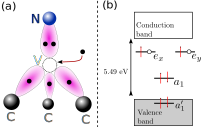
\includegraphics[width=0.8\textwidth]{Figures/NV_electrons}
\caption{(a) Representation of the nitrogen and carbon orbitals surrounding the vacancy of an NV center. Each black dot represents an electron. A sixth electron is required to form the negatively charged NV$^-$ state. (b) Molecular orbitals of the NV center predicted from the the $C_{3v}$ symmetry of the defect. The electron occupation of the NV$^-$ ground state is represented by red arrows.}
\label{NV electrons}
\end{figure}

We will first cover the molecular aspect of the NV defect in diamond and the energy levels of the defect predicted from group theory and ab initio computations.

Fig. \ref{NV electrons}-a) illustrates the $sp^3$ orbitals of the carbons and nitrogen atoms neighboring the vacancy, as well as the 5 electrons occupying dangling bonds from these atoms and a sixth electron captured to form the negatively charged NV$^-$ state. 

Fig. \ref{NV electrons}-b) shows the predicted molecular orbitals of the NV centers, initially computed as linear combination of the $sp^3$ orbitals respecting the $C_{3v}$ symmetry of the defect \citep{loubser1978electron}. This model has since been confirmed by ab initio computation and experimental observations \citep{doherty2013nitrogen}. In particular ab initio computations have shown that the molecular orbitals of the NV center are mostly localized on the nearest neighbors of the vacancy \citep{gali2008ab}. Ab initio computation has also determined that the $a'_1$ level lies in the valence band and is thus often ignored.

The electron occupations shown in Fig. \ref{NV electrons}-b) corresponds to the electronic ground state of the NV$^-$ charge state.

In the remaining part of this manuscript, we will only consider the negatively charged NV$^-$ state, unless specified otherwise. We will therefore omit the ``$-$" and simply refer to the negatively charged state as ``NV".
\subsection{Optical properties of the NV center}
\begin{figure}[h!]
\centering
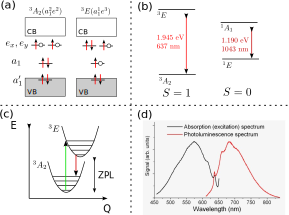
\includegraphics[width=1\textwidth]{Figures/NV_optical}
\caption{Optical properties of the NV center. (a) Electron occupation of the molecular orbitals for the electronic ground state $^3A_2$ and the first excited state $^3E$. (b) Diagram of the main optical transition between the two spin triplet states and of the IR transition between the two singlet sates. The value of the transition corresponds to the zero phonon line (ZPL) and are taken from \citep{doherty2013nitrogen}. (c) Representation of the vibronic structure for the $^3A_2$ and $3^E$ states under the Franck-Condon approximation. The graph axes are the energy of the states E and configuration coordinate q. The green and red arrow represents non-resonant (Stokes) absorption and emission. (d) Emission and absorption spectrum of the NV center main transition at 300 K, from PL and PLE measurements respectively. Credits: Wikimedia commons}
\label{NV optical}
\end{figure}

Because the NV center has discrete electronic transitions inside the diamond band gap, it fluoresces: it can absorb light from $450-650$ nm and re-emits light in the $600-800$ nm band.

Fig. \ref{NV optical} explains the origin of the NV center optical properties. Fig. \ref{NV optical}-a) illustrates the electronic ground state $^3A_2$ and first excited state $^3E$, where 1 electron from the $a_1$ molecular orbital is promoted to the $e$ level. Both of these electron occupations have two unpaired electrons, meaning that they can exist either either in a spin triplet state ($S=1$) or a spin singlet state ($S=0$) \footnote{The two singlet states $^1E$ and $^1A_1$ represented in Fig. \ref{NV optical}-b) are both of configuration $a_1^2e^2$ where the two $e$ electrons are either in a the same $e$ orbital, or in an antisymmetric superposition of the two $e$ orbitals \citep{doherty2011negatively}.}. 

Fig. \ref{NV optical}-b) shows the zero phonon line (ZPL) for the main transition of the triplet ($^3A_2$ and $^3E$) and singlet ($^1E$ and $^1A_1$) states. It should be noted that due to an inter system crossing between the $^1E$ and $^3A_2$ levels, excitation or absorption of the singlet transition is only possible with a conjoint excitation of the triplet states. By default, we refer to the NV center photoluminescence (PL) as the emission between the two triplet states.

Fig. \ref{NV optical}-c) illustrates the vibronic structure of the $^3A_2$ and $^3E$ states under the Franck-Condon approximation \citep{gali2011time}. The emission and absorption of light associated with the triplet transition can be accompanied by the emission or absorption of an optical phonon. Because the lifetime of the optical phonons is very short, the absorption or emission of light almost always start from the fundamental state of the $^3A_2$ and $^3E$ level, which explains why the absorption of light can only be done for energies above the ZPL, and the emission for energies below the ZPL (Stokes process).

Finally Fig. \ref{NV optical}-d) shows the absorption and emission spectrum of NV centers at 300 K. A weak zero-phonon-line is visible at 637 nm, with large phonon sidebands in emission and absorption.

\medskip
Compared to similar solid state photon sources (other color centers, quantum dots, dye molecules...), the NV center offer several advantages. First, they are very bright thanks to the $\sim 11\ \rm ns$ lifetime of the excited state and quantum efficiency of $0.7-0.8$ \citep{schirhagl2014nitrogen}. With proper nanophotonics engineering (solid immersion lenses or diamond waveguide) the PL collected from a single NV center can reach a few $10^6$ photons/s \citep{schroder2016quantum}.  Secondly, the NV center is also extremely photostable under green excitation, and does not show any photobleaching \citep{brouri2000photon}. Finally, the diamond itself is resistant to heat and chemical attacks, and presents low toxicity for biologic systems \citep{fu2007characterization}. There are however drawbacks in using NV centers for photonics applications, the main one being that $\leq 4\%$ of the photons emitted by the NV centers are in the ZPL (low Debye Waller factor), even at cryogenic temperature \citep{johnson2015tunable}. This limits the potential of NV centers for quantum photonic devices \citep{bradac2019quantum}.

\subsection{Spin properties of the NV center electronic ground state}
\begin{figure}[h!]
\centering
\includegraphics[width=1\textwidth]{Figures/spin_fine_hyperfine}
\caption{Representation of the fine and hyper-fine structure of the $^3A_2$ state for a $^{14}N$ nucleus and $^{12}C$ nuclei.}
\label{NV spin}
\end{figure}

We will only focus here on the spin structure of the electronic ground state $^3A_2$, as the lifetime of the other states is too short to make effective spin qubits. All the numerical values in this section were found in \citep{smeltzer2009robust, doherty2013nitrogen} and the references within.

The spin structure in the ground state consists in an electronic spin $S=1$ coupled to the nuclear spin of the nearby nuclei. Carbon's most common isotope is $^{12}C$ at 98.9 \% natural abundance. $^{12}C$ has a a nuclear spin $I=0$ and therefore does not contribute to the hyper-fine structure. Nitrogen's most common isotope however is $^{14}N$ at 99.6 \% natural abundance which has a nuclear spin $I=1$ and does create a hyper-fine splitting. We will only cover here the most likely configuration for an NV center which is a $^{14}N$ nucleus and $^{12}C$ nuclei as closest neighbors. 

The spin system considered is then an electronic spin $S=1$ coupled to a nuclear spin $I=1$ with a Hilbert space of dimension $(2S+1)(2I+1)=9$. The spin Hamiltonian of the system can be written:
\begin{equation}
\mathcal{H}=\mathcal{H}_e + \mathcal{H}_n + \mathbf{S}\cdot \bar{\bar{A}}\cdot \mathbf{I},
\end{equation}
where $\mathcal{H}_e$ is the purely electronic spin Hamiltonian, $\mathcal{H}_n$ the purely nuclear spin Hamiltonian, $\mathbf{S}$ the electronic spin operator, $\mathbf{I}$ the nuclear spin operator and $\bar{\bar{A}}$ the hyper fine tensor.
\subsubsection{Electronic spin Hamiltonian}
The electronic spin $\mathcal{H}_e$ can be written:
\begin{equation}
\label{eq. spin elec}
\mathcal{H}_e=D S_z^2 + \gamma_e \mathbf{S} \cdot \mathbf{B} + \mathcal{H}_{elec}(\mathbf{E})+ \mathcal{H}_{strain}(\mathbf{\bar{\bar{\varepsilon}}}).
\end{equation}

The term $D S_z^2$ corresponds to the fine structure of the electronic spin. It originates from the dipole-dipole coupling between the two unpaired electrons of the defect. Due to the strong anisotropy of the molecular orbitals of the defect, the fine structure term imposes the quantization axis $\mathbf{z}$ (via the $S_z$ operator) where $\mathbf{z}$ is the direction of the N$-$V axis in the diamond. $D$ is called the zero field splitting (ZFS) factor and its value is $D\approx 2.87\ \rm GHz$ at 300 K.

$\gamma_e \mathbf{S} \cdot \mathbf{B}$ is the Zeeman splitting of the spin, where $\gamma_e \approx 2.8\ \rm MHz/G$ is the gyromagnetic ratio of the electronic spin (almost equal to that of a free electron in the case of the NV center).

$\mathcal{H}_{elec}$ and $\mathcal{H}_{strain}$ are the dependency of the Hamiltonian on the electric field and crystal strain and will be discussed in further details in chapter 4.

\subsubsection{Nuclear spin Hamiltonian and hyperfine coupling}
The nuclear spin $\mathcal{H}_n$ can be written:
\begin{equation}
\mathcal{H}_e=Q I_z^2 + \gamma_n \mathbf{I} \cdot \mathbf{B},
\end{equation}

where $Q=-4.945\ \rm MHz$ is the nucleus electric quadrupole moment and $\gamma_n=0.308\ \rm kHz/G$ is the nuclear gyromagnetic ratio.

Finally the hyper-fine tensor can be written diagonally:
\begin{equation}
\bar{\bar{A}} = \begin{pmatrix}
A_{xx} & 0 & 0 \\
0 & A_{yy} & 0 \\
0 & 0 & A_{zz}
\end{pmatrix},
\end{equation}
where $A_{zz}=-2.162\ \rm MHz$ and $A_{xx}=A_{yy}=-2.62\ \rm MHz$. The $z$ direction in the electronic spin Hamiltonian, the nuclear spin Hamiltonian and the hyper-fine tensor awlays refer to the direction of the N$-$V axis.

Fig. \ref{NV spin} illustrates the fine and hyper-fine structure of the NV center without any external fields.

For most intent and purposes, the hyper-fine structure of the NV center can simply be thought of as an energy offset, and is thus often ignored. The electric and strain dependencies of the electronic Hamiltonian are also often ignored as they are of second order compared to the magnetic field dependency. This leads to the simpler spin Hamiltonian:

\begin{align}
\label{NV spin Hamiltonian basic}
\mathcal{H}&=D S_z^2 + \gamma_e \mathbf{S} \cdot \mathbf{B} \\
&=\begin{pmatrix}
D-\gamma_e B_z & \frac{\gamma_e (B_x+iB_y)}{\sqrt{2}} & 0 \\
\frac{\gamma_e (B_x-iB_y)}{\sqrt{2}} & 0 & \frac{\gamma_e (B_x+iB_y)}{\sqrt{2}} \\
0 & \frac{\gamma_e (B_x-iB_y)}{\sqrt{2}} & D+\gamma_e B_z
\end{pmatrix}
\end{align}

\bigskip
The NV center's spin usage as a qubit is prevalent in quantum communication \citep{wehner2018quantum}, quantum computing \citep{de2021materials} and quantum sensing \citep{degen2017quantum}. Part of the reason for this wide usage are the overall long relaxation times (lifetime $T_1$ and coherence time $T_2$) of the order of a few ms at room temperature \citep{balasubramanian2009ultralong}, as well as the ability to address individual nuclear spins with even longer relaxation times \citep{awschalom2018quantum}. However the main advantage of the NV center spin compared to other solid state spin qubits is its ability to be polarized and read-out optically thanks to the properties detailed in the following section.


\subsection{Spin and optical levels intersystem crossing}
\label{sec ISC}
\begin{figure}[h!]
\centering
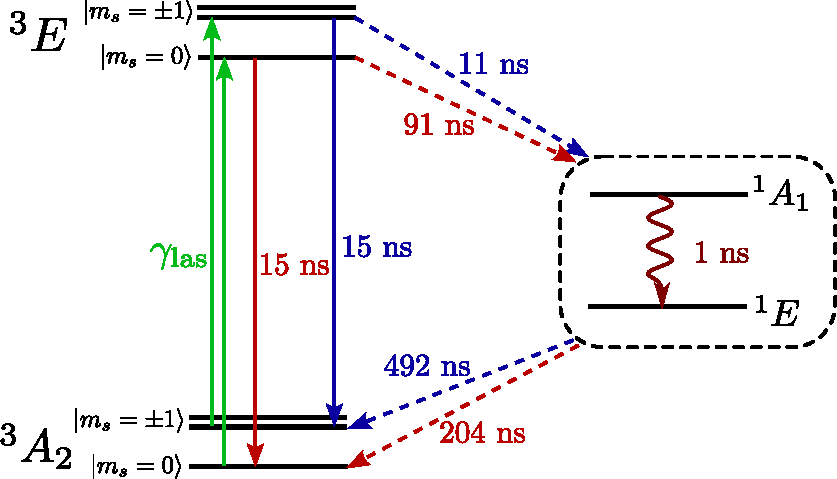
\includegraphics[width=0.8\textwidth]{Figures/ISC}
\caption{Inter system crossing of the NV center. Blue arrows symbolize decay channels to and from the $\ket{m_s=\pm 1}$ states and red arrows the decay channels to and from the $\ket{m_s=0}$ states. Green arrows symbolize the optical excitation induced by the laser. The times indicated correspond to the inverse of the decay rates found in \citep{gupta2016efficient}.}
\label{ISC}
\end{figure}

The optical excitation and radiative decay between the $^3A_2$ and $^3E$ levels preserve the spin projection $m_s$ \citep{robledo2011spin}. There is however a non-radiative decay path which involves in inter-system crossing with the singlet states $^1A_1$ and $^1E$ that depends on the the triplet states spin projection.

Fig. \ref{ISC} summarizes the possible decay channels from the $^3E$ states. We assume that the electrons are initially excited from the $^3A_2$ states via a green laser with a rate $\gamma_{\rm las}$. The $^3E$ states can then either decay radiatevely and emit a 600$-$800 nm photon, or undergo an intersystem crossing and decay through the singlet states. We consider the decay channel through the singlet state as non-radiative due to the strong non radiative channels competing with the IR radiative transition (quantum efficiency $\leq 10^{-3}$ for the singlet transition \citep{rogers2008infrared, ma2010excited, acosta2010optical}).

The rates $\gamma$ of the various decay processes, represented in Fig. \ref{ISC} by the time constant $\tau=1/\gamma$, strongly depends on the spin projection $m_s$: the likeliness to undergo a non-radiative decay is $\sim 4$ times\footnote{$\frac{15+91}{15+11}\approx 4$} more likely when starting from the $\ket{\pm 1}$ states than when starting from the $\ket{0}$ state. Similarly, the singlet state is $\sim 2.4$ times\footnote{$\frac{492}{204} \approx 2.4$} more likely to decay in the $\ket{0}$ state than in the $\ket{\pm 1}$ states.

These spin selective intersystem crossings mean that an optical pumping scheme in the $\ket{m_s=0}$ spin state takes place under constant green excitation. At optical saturation, the polarization of the $\ket{0}$ state can reach $70-90\ \%$ \citep{gupta2016efficient}, which is equivalent to a thermal polarization (for B=0) with a spin temperature of $\approx 65\ \rm mK$ \footnote{\begin{equation*}
T=\frac{h D}{k_B \ln (\frac{1-P}{2P})} \approx 65\ \rm mK,
\end{equation*}
where $D$ is th ZFS factor described in eq. (\ref{eq. spin elec}) and $P\approx 0.8$ is the spin polarization defined as the population in the $\ket{0}$ state.} while the diamond itself can remain at room temperature.

Another effect of the intersystem crossing is the ability to optically readout the spin state of the NV center: since the $\ket{0}$ state is more likely to undergo a radiative decay than the $\ket{\pm 1}$ states, the expected photoluminescence (PL) is higher when starting from the $\ket{0}$ state than a $\ket{\pm 1}$ state. While the $\ket{+1}$ and $\ket{-1}$ states cannot be a priori distinguished, a direct excitation of the $\ket{+1} \to \ket{0}$ or $\ket{-1} \to \ket{0}$ transition with a resonant microwave can unambiguously reveal the initial spin state.

It should be noted that the decay rates indicated in Fig. \ref{ISC} cannot be directly measured. They have to be inferred from the PL dynamics at short times after illumination. Different experiments and different models have thus lead to different decay rates \citep{duarte2021effect}. 


\section{Basic operations with NV centers}

This section introduces two elementary operations with NV centers that are Rabi oscillations and optically detected magnetic resonance (ODMR).

Rabi oscillations is the basis for any kind of coherent qubit manipulation while ODMR is used to find the transition frequencies of the NV centers, as well as being a basic magnetometry protocol.

This section also covers the experimental setup used for these two operations and for many other NV experiments, as well as the concept of longitudinal and transverse magnetic field with regard to the NV principal axis.

\subsection{Experimental setup}
\begin{figure}[h!]
\centering
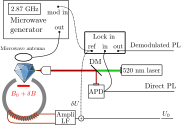
\includegraphics[width=0.8\textwidth]{Figures/shema_exp}
\caption{Confocal microscopy setup detailed in main text}
\label{setup}
\end{figure}
The three most common experimental degrees of freedom to consider for NV experiments are: the optical illumination, the microwave field and the external magnetic field. Other parameters such as the crystal temperature, the electric field or the crystal stress can also be controlled for specific applications.

Fig. \ref{setup} shows a multi-purpose experimental setup which offers a control over these three degree of freedoms. Unless specified otherwise, this is the experimental setup that was used to perform all the measurements shown in this manuscript. 

The setup consists of a confocal microscope where the excitation from a green laser (Thorlabs CPS532, 532 nm, 5 mW) is focused on a sample containing NV centers with a microscope objective (NA $\sim$ 0.5). The NV PL is then collected by the same objective and isolated from the back-scattered laser light with a dichroic mirror (DM) and additional filters (532 nm notch filter and 645 nm longpass filter to filter out the NV$^0$ PL). The PL is collected on an avalanche photodiode (Thorlabs APD410A or Perkin Elmer SPCM-AQRH-15) whose signal is sent to the acquisition card (NI X-series).

The laser beam goes through an acousto-optic modulator (AOM, AA opto-electronic) controlled externally to create arbitrary light pulses (resolution $\sim$ ns). The microwave field is generated by a Rhode \& Shwarz SMB 100A generator and emitted with a home-made loop antenna positioned at $<$ 1 mm of the sample. A microwave switch (Mini-circuits ZASWA-2-50DRA+) is used to create microwave pulses (resolution $\sim$ 10 ns). The control pulses for the AOM and the microwave switch are generated either by the NI X-series card (resolution $\sim$ 1 $\mu$s), or by a pulseblaster ESR-PRO (resolution $\sim$ 10 ns). The microwave field can be amplified with a Mini-circuits ZHL-5W-422+ amplifier to achieve higher Rabi frequencies. 

Finally the magnetic field is generated either with a permanent magnet (up to $\sim$ 200 mT) or with a homemade electromagnet (up to $\sim$ 30 mT) alimented via a low freqency amplifier (Leybold power function generator 522663). Both the permanent magnet and the electromagnet can be  attached to a rotation stage for precise alignment.
\subsection{Rabi Oscillations}
\begin{figure}[h!]
\centering
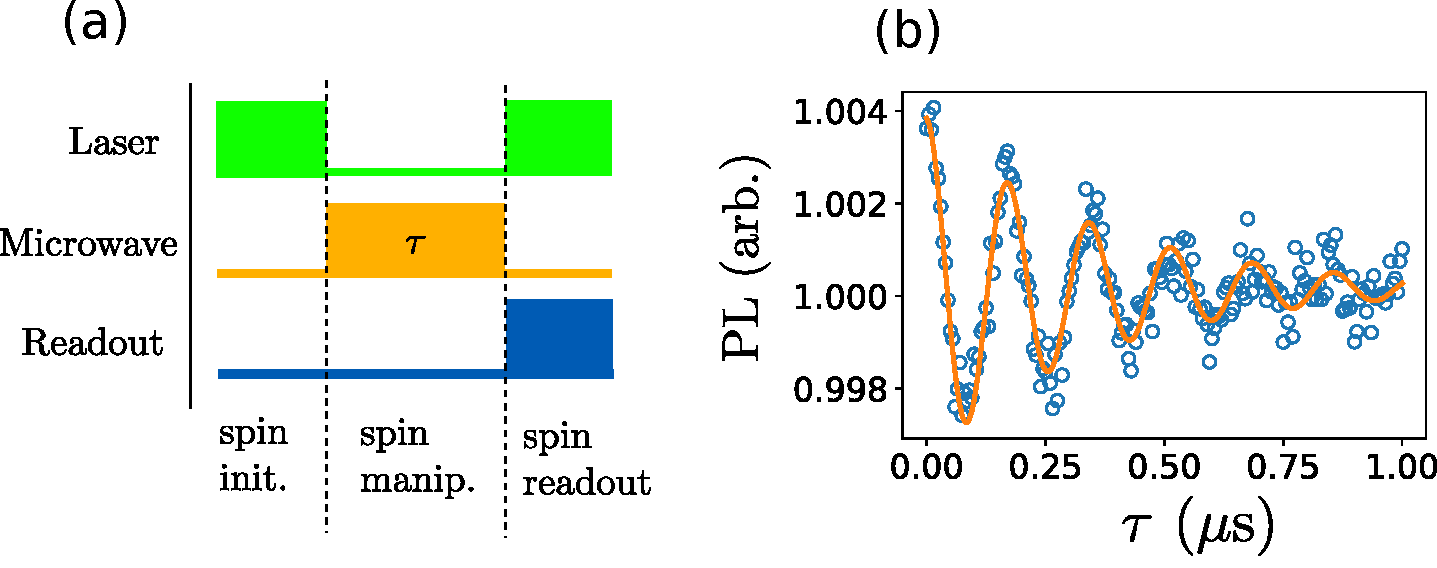
\includegraphics[width=\textwidth]{Figures/Rabi}
\caption{Rabi oscillations. (a) pulse sequence used to measure Rabi oscillations. (b) Experimental data on sample CVD-pink (cf samples [REF]).}
\label{Rabi}
\end{figure}

The general technique for experiments involving NV spins proceeds as follow: 
\begin{itemize}
\item First the spins are polarized. This is done with a green laser pulse ($1-100$ $\mu$s depending on the laser intensity) which polarizes the spins in the $\ket{m_s=0}$ state at $\sim$ 80 \%.
\item  Then the spins are manipulated. This process often involves a microwave field resonant with one of the spin transitions.
\item Finally the spins are read out. The simplest spin readout for NV centers consists in looking at the PL right after the laser is turned on: if the spin was in the $\ket{m_s=0}$ state, the initial PL will be high, whereas if the spin was in a $\ket{m_s=\pm 1}$ state, the initial PL will be low. For longer exposure time, the spins end up re-polarized in the $\ket{m_s=0}$ state and no information can be gained on the initial spin state anymore. The optimal readout time is of the same order as the spin polarization time ($1-100$ $\mu$s).
\end{itemize}

Fig. \ref{Rabi}-a) shows the pulse sequence used to observe Rabi oscillations with NV centers. In this case, the spins manipulation simply consists in a microwave pulse of variable duration $\tau$. The microwave frequency or the magnetic field needs to be adjusted so that at least one NV spin transition (either $\ket{0} \to \ket{+1}$ or $\ket{0} \to \ket{-1}$) is resonant with the microwave field. 

Fig. \ref{Rabi}-b) shows the result of such an experiment on a spin ensemble. The PL signal oscillations correspond to the oscillations of the spin population between the bright $\ket{0}$ state and the dark $\ket{-1}$ state. For long microwave pulses ($>$ 1 $\mu$s typically), the spins reach a steady state with  $\sim$ 50 \% population in both the $\ket{0}$ and $\ket{-1}$ states.


\subsection{Optically detected magnetic resonance}
\begin{figure}[h!]
\centering
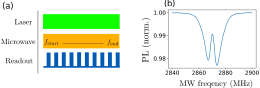
\includegraphics[width=\textwidth]{Figures/ODMR_basique}
\caption{ODMR protocol. (a) Pulse sequence used for CW ODMR: the microwave is kept on during the whole sequence while the frequency is scanned from $f_{\rm start}$ to $f_{\rm end}$. (b) ODMR spectrum with no magnetic field on sample ADM-15-4.}
\label{ODMR basique}
\end{figure}

Optically detected magnetic resonance (ODMR) is the most commonly employed magnetometry protocol with NV centers due to its simplicity and the fact that it does not require prior calibration.

The protocol for continuous wave (CW) ODMR is presented in Fig. \ref{ODMR basique}. In this simple protocol, the microwave is always turned on while the frequency spans a predefined interval $[f_{\rm start}, f_{\rm end}]$. The PL is recorded as the microwave is being swept, with a typical acquisition time for each PL sample $> 1\ \rm ms$. The sweeping frequency must be slow enough so that the PL can reach a steady state with the microwave field for each sample acquisition. 

As we saw in the last section, the steady state of the NV center spin with a resonant microwave field is a statistical mixture of 50 \% $\ket{0}$ and 50 \% $\ket{\pm 1}$ \footnote{We are assuming here that the Rabi frequency is greater than the laser polarizing rate, which is often the case in practice}. If the microwave field is not resonant with a spin transition however, the steady state is predominantly $\ket{0}$ due to the spin polarization caused by the laser. The NV PL will therefore be lowered when the scanning microwave field becomes resonant with one of the NV spin transitions. 

Fig. \ref{ODMR basique}-b) shows an example of ODMR spectrum on an NV ensemble with no external magnetic field. The reason for the two bumps instead of a single one centered on $D=2870\ \rm MHz$ is the splitting of the $\ket{+1}$ and $\ket{-1}$ levels occasioned by the strain and local electric field, which will be further discussed in chapter 4.

\subsubsection{ODMR with lock-in detection}
\begin{figure}[h!]
\centering
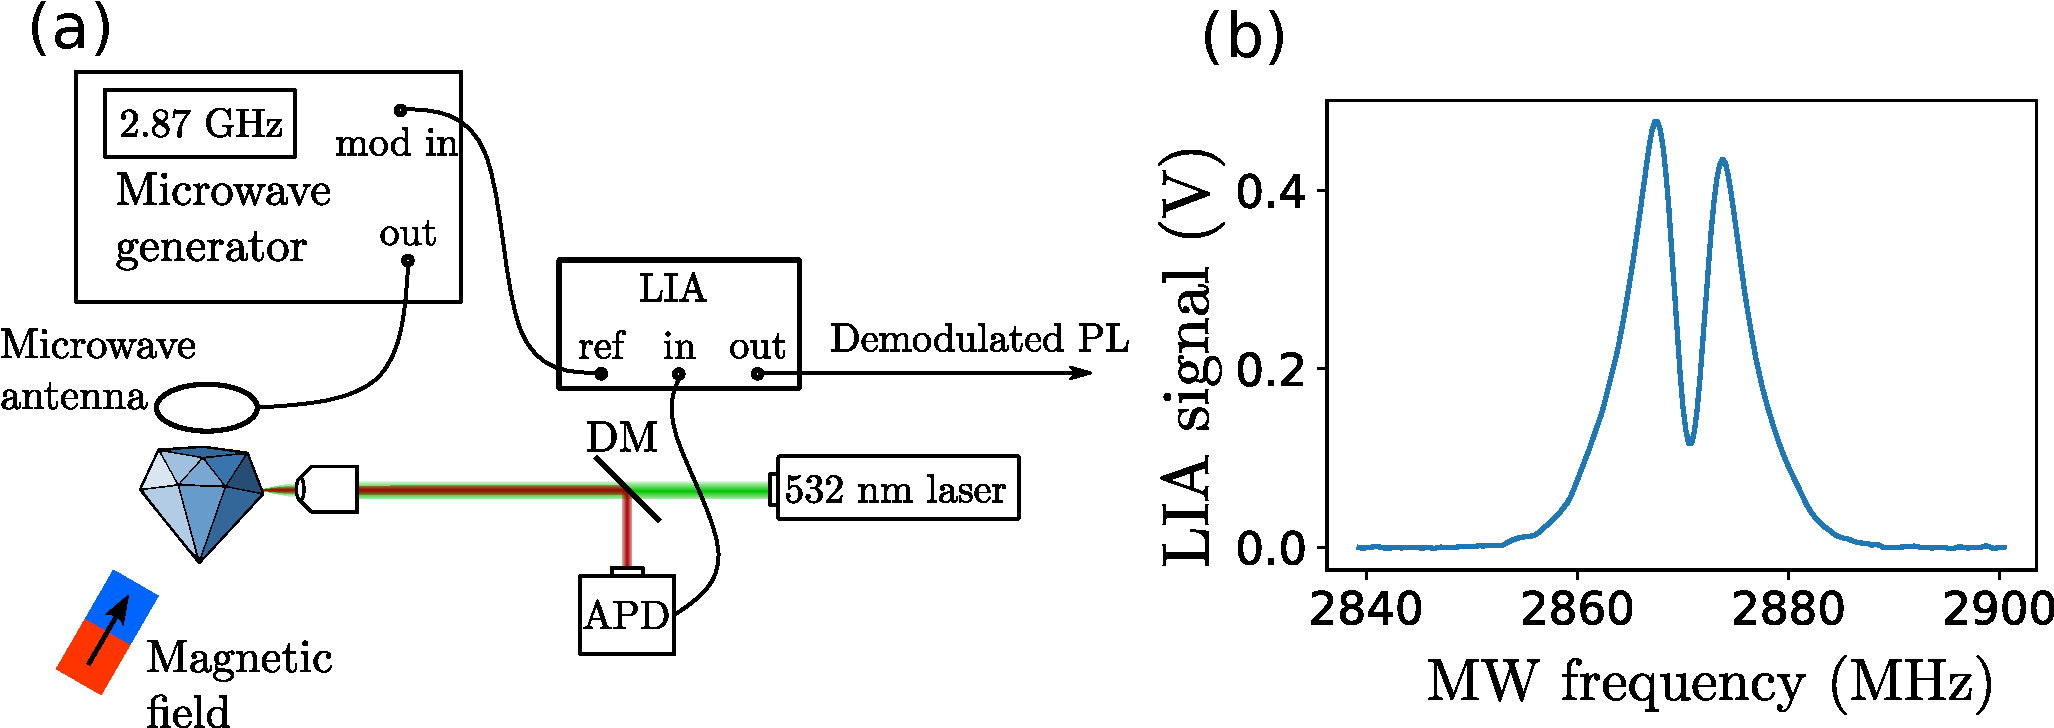
\includegraphics[width=\textwidth]{Figures/ODMR_lockin}
\caption{ODMR protocol with lock-in detection. (a) Simplified confocal microscope setup with a lock-in amplifier (LIA) modulating the mircowave and demodulating the PL. (b) Demodulated ODMR spectrum with no magnetic field on sample ADM-15-4.}
\label{ODMR lockin}
\end{figure}


Because the ODMR protocol delivers a continuous signal (the PL) as a function of a periodic excitation (the microwave field), it is well suited to amplitude or frequency modulation and lock-in detection. 

The principle of lock-in detection will not be covered here, the key idea is that lock-in detection allows to translate the signal spectrally in a region less prone to noise. In this case, the ODMR signal is a DC measurement and is therefore prone to slow freqency noises such as thermal or mechanical drifts and laser amplitude fluctuations. The microwave field can thus be modulated (in amplitude, frequency or phase) at a frequency fast enough to mitigate the low freqency noises, but slow enough compared to the NV photodynamics. 

Fig. \ref{ODMR lockin}-a) shows the ODMR lock-in setup, and Fig. \ref{ODMR lockin}-b) shows an example of ODMR spectrum with microwave amplitude modulation. All the lock-in spectra shown in this manuscript were produced with 100 \% amplitude modulation at a frequency $f_{\rm mod} \sim 1\ \rm kHz$.

\subsection{ODMR with NV ensemble: longitudinal and transverse magnetic field}

\begin{figure}[h!]
\centering
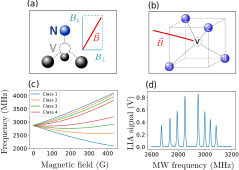
\includegraphics[width=\textwidth]{Figures/ODMR_8_classes}
\caption{(a) Geometry of the NV center and definition of $B_z$ and $B_\perp$. (b) Representation of the 4 possibles orientations (``classes") of the N$-$V axis, corresponding to the 4 $\langle 111 \rangle$ directions of the diamond cubic cell. (c) Simulation of the evolution of the transition frequencies for each class of NV centers as a function of the amplitude of the applied magnetic field ($\textbf{B}$ orientation chosen arbitrarily). (d) ODMR spectrum on sample ADM-150-1 for a magnetic field of $\sim 90\ \rm G$.}
\label{ODMR 8 classes}
\end{figure}

We mentioned previously that the NV spin Hamiltonian (eq. (\ref{NV spin Hamiltonian basic})) was anisotropic due to the fine structure term $D S_z^2$ where $z$ is the direction of the N$-$V axis in the crystal. The magnetic field is thus often decomposed between the longitudinal magnetic field $B_z$ and the transverse magnetic field $B_\perp=\sqrt{B_x^2+B_y^2}$ (see Fig. \ref{ODMR 8 classes}-a). 

For weak magnetic fields ($\gamma |\textbf{B}| \ll D$), the energy of each of the three spin Hamiltonian eigenstates $\ket{0}$, $\ket{+1}$ and $\ket{-1}$\footnote{The notation of $\ket{0}$, $\ket{\pm 1}$ to designate the spin Hamiltonian eigenstates is slightly abusive as $S_z$ does not commute with $\mathcal{H}$ when $B_\perp \neq 0$. The true eigenstates however remain close to $\ket{0}$, $\ket{\pm 1}$ as long as $\gamma_e B_z > \frac{(\gamma_e B_\perp)^2}{D}$.} can be approximated in a perturtbative approach to: %cf AN.py
\begin{align}
\nu_0&= -\frac{(\gamma_e B_\perp)^2}{D} \\
\nu_{-1} &= D - \gamma_e B_z + \frac{(\gamma_e B_\perp)^2}{2D} \\
\nu_{+1} &= D + \gamma_e B_z + \frac{(\gamma_e B_\perp)^2}{2D}
\end{align}

Fig. \ref{ODMR 8 classes}-b) represent the 4 possible orientation of the N$-$V axis in a diamond single crystal. We refer to these orientations as ``classes" since NV centers belonging to the same class will perceive the same transverse and longitudinal magnetic field, and thus will have the same spin Hamiltonian. For large NV ensembles (a confocal spot can contain more than $10^9$ NV centers in dense ensemble), we can consider that each class is equally represented \footnote{It is possible to create NV centers with a preferential orientation \citep{lesik2014perfect} but this requires specific conditions during the growth process of the diamond} and that each class is responsible for two lines in the ODMR spectrum (one for the $\ket{0} \to \ket{-1}$ transition and one for the $\ket{0} \to \ket{+1}$ transition). 

Fig. \ref{ODMR 8 classes}-c) shows a simulation of the evolution of the transition frequencies $\nu_{+1} - \nu_{0}$ and $\nu_{-1} - \nu_{0}$ for all 4 classes as a function of the magnetic field amplitude, with the magnetic field orientation fixed in an arbitrary direction. Fig. \ref{ODMR 8 classes}-d) shows an ODMR spectrum with NV ensembles. 8 lines are visible corresponding to the two transitions of the 4 classes. Based on the position of these 8 lines, it is possible to determine the projection of the magnetic field on each of the 4 N$-$V axes, and thus to reconstruct the full 3D magnetic field with respect to the diamond crystalline axes.

We should also note that the state mixing caused by the transverse magnetic field deteriorates the polarization scheme detailed in Sec. \ref{sec ISC}. For strong transverse magnetic fields ($\gamma_e B_\perp \sim D$), the optical polarization is almost completely quenched, which prevents any kind of coherent NV manipulation \citep{tetienne2012magnetic}.

\section{Dynamics of the NV center spin}

This section focuses on the dynamics of the NV spin, and more specifically on its various relaxation times. Relaxation times are important properties of spin qubits as they often are the limiting factor for quantum information or quantum sensing applications \citep{de2021materials, degen2017quantum}.

The relaxation times are generally decomposed between the longitudinal relaxation time $T_1$ which corresponds to the characteristic time of the return to thermal equilibrium for the populations (diagonal elements of the density matrix), and the transverse relaxation time $T_2$\footnote{We follow here the NMR nomenclature} which corresponds to the relaxation of the spin state coherences (non diagonal elements of the density matrix).

The transverse relaxation time, also called coherence time or dephasing time, is often further decomposed between the inhomogeneous dephasing time $T_2^*$ and the homogeneous dephasing time $T_2$. The $T_2^*$ time includes inhomogeneous dephasing processes such as the inhomogeneity in space (when multiple qubits are probed) and time of the external fields. The $T_2$ time corresponds to the coherence time where some of these inhomogeneities have been corrected, for instance with a Hanh echo sequence \citep{hahn1950spin} or a dynamical decoupling scheme \citep{naydenov2011dynamical}. While $T_2^*$ is an intrinsic property of the sample studied, $T_2$ depends on the rephasing scheme used. More careful nomenclatures will label the $T_2$ times as $T_{2,\rm echo}$ or $T_{2,\rm DD}$ \citep{de2021materials} for instance. The relaxation times are ordered as follows:
\begin{equation}
T_2^* < T_2 < 2 T_1.
\end{equation}

The relaxation times of NV centers depend mainly on their environment, and can vary by several order of magnitude depending on the sample used. The following paragraphs will cover the measurement processes of the different relaxation times and the typical values for the samples used in this manuscript.

\subsection{NV spin $T_1$}
\label{sec T1 NV}
\subsubsection{Measurement protocol}
\begin{figure}[h!]
\centering
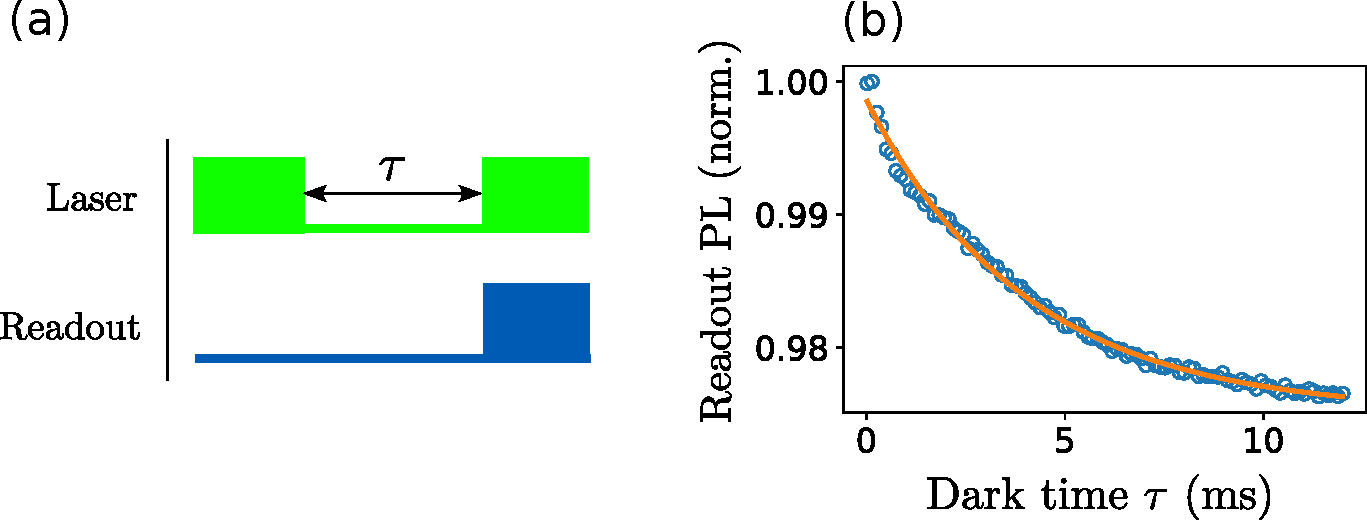
\includegraphics[width=\textwidth]{Figures/T1_basique}
\caption{Basic $T_1$ measurement scheme. (a) Pulse seqeunce used. (b) Experimental data obtained on sample CVD-pink for low laser intensity. The orange line corresponds to an exponential fit with time constant $\tau=4.0\ \rm ms$.}
\label{T1 basique}
\end{figure}


$T_1$ is the simplest relaxation time to measure because the spin populations are directly correlated to the NV centers PL. Fig. \ref{T1 basique} shows the pulse sequence used and an experimental result of the $T_1$ sequence. The spin lifetime $T_1$ is one of the only spin property that can be measured without a resonant microwave.

The sequence shown in Fig.\ref{T1 basique} can be improved by implementing a common mode rejection technique described in Fig. \ref{T1 soustraction}-a). This protocol works as follow: first, a basic $T_1$ sequence is recorded, which we will denote $S_1$. Then the sequence is repeated with an additional $\pi$-pulse on one the NV transitions right before the readout. This $\pi$-pulse will project the remaining $\ket{0}$ population difference into a $\ket{\pm 1}$ state. The second readout is labeled $S_2$, and the final spin state readout is $S_1 -S_2$ which rejects every contribution to the PL outside of the spin relaxation. 



Fig. \ref{T1 soustraction}-b) shows the experimental result of the $S_1$ and $S_2$ sequences on the same sample that was used in Fig. \ref{T1 basique}. The difference between the $S_1$ data in Fig. \ref{T1 soustraction}-b) and the the data in Fig. \ref{T1 basique}-b) comes from the laser intensity used. In Fig. \ref{T1 soustraction}, the laser intensity was high enough ($> 1\ \rm{mW}$) that photoionization between NV$^-$ and NV$^0$ becomes significant. Furthermore, for dense ensemble, a charge recombination mechanism operates even in the dark \citep{giri2018coupled, giri2019selective} (most likely due to charge tunneling between impurities \citep{choi2017depolarization}) . On the other hand, the laser intensity used in Fig. \ref{T1 basique} was small enough ($< 10\ \mu \rm{W}$) that the charge state state photodynamics contribution was negligible compared to the spin depolarization.

Fig. \ref{T1 soustraction}-c) Shows the subtraction of the $S_1$ and $S_2$ signal. Despite the complex shape of the initial $S_1$ and $S_2$ signals, $S_1-S_2$ is nicely fitted with an exponential decay similar to the results found in Fig. \ref{T1 basique}.

\begin{figure}[h!]
\centering
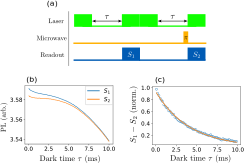
\includegraphics[width=\textwidth]{Figures/T1_protocole_soustraction}
\caption{Common mode rejection $T_1$ measurement scheme. (a) Pulse seqeunce used. (b) PL signals $S_1$ and $S_2$ obtained on sample CVD-pink with a high laser intensity. (c) Subtraction $S_1-S_2$ versus dark time $\tau$. The experimental data is fitted with an exponential decay of time constant $\tau=4.1\ \rm ms$.}
\label{T1 soustraction}
\end{figure}

The photodynamics of the NV charge state is a complex subject which is still actively researched \citep{craik2020microwave, gorrini2021long}. The common mode rejection scheme described  here is often employed with dense ensemble of NV centers \citep{jarmola2012temperature, mrozek2015longitudinal, choi2017depolarization} as it allows to completely bypass the charge dynamics.

\subsubsection{Physical origin and typical values}

We distinguish three different origin for the the $T_1$ relaxation process:
\begin{itemize}
\item \textbf{Spin-phonon relaxation:} the spin states are weakly coupled to the crystal phonon bath through spin-spin and spin-orbit interactions \citep{norambuena2018spin}, which can result in a phonon-induced spin relaxation. The dominant relaxation mechanism depends on the  temperature regime, with the two-photon Raman process believed to be dominant at room temperature \citep{takahashi2008quenching, jarmola2012temperature} while the dominant process as at cryogenic temperature ($4\sim100$ K) is believed to be a two phonons Orbach process \citep{redman1991spin, norambuena2018spin}. The spin-phonon relaxation time strongly depends on the crystal lattice temperature, with relaxtion times of the order $T_1 \sim 5\ \rm ms$ at room temperature, and up to 8 hours at for mili-K temperatures \citep{astner2018solid}.

\item \textbf{Electric and magnetic field noises:} both electric and magnetic fields can directly excite the $\ket{0} \to \ket{\pm 1}$ spin transition \citep{udvarhelyi2018spin}. As a result, magnetic and electric field noise can reduce the spin $T_1$ if their spectrum overlap with the NV transitions. This is particularly important for near surface spins because of the strong noise caused by electronic defects on the surface \citep{sangtawesin2019origins}. The $T_1$ of near surface NV center can be as low as $\sim 10\ \mu$s, but the surface effects are only effective at very short range (within $\sim 10\ \rm nm$ of the surface).

\item \textbf{Resonant dipolar interaction with other paramagnetic impurities:} Dipolar interaction betwen two spins will be detailed more thoroughly in the following section. Dipole-dipole interaction between NV centers and surrounding spins is responsible for both transverse and longitudinal spin relaxation, with the added condition of energy matching (resonance) for longitudinal relaxation. The $T_1$ time associated with dipole-dipole interaction strongly depends on the spin concentration and can be as low as $\sim 25 \mu$s \citep{hall2016detection}.
\end{itemize}

All the measurements shown in this manuscript were performed at room temperature. The spin-phonon interaction thus creates a baseline value for the NV $T_1$ time at $\sim 5\ \rm ms$. Every sample studied were at least a few $\mu$m thick and we will therefore neglect the surface noise contribution in our analyses. The dipole-dipole induced relaxation however is of crucial importance for the next chapters, where it will be further detailed. $T_1$ times between $0.1 \sim 1\ \rm ms$ were routinely observed for samples with high NV concentration.

\subsection{NV spin $T_2^*$}
\subsubsection{Measurement protocol}
\begin{figure}[h!]
\centering
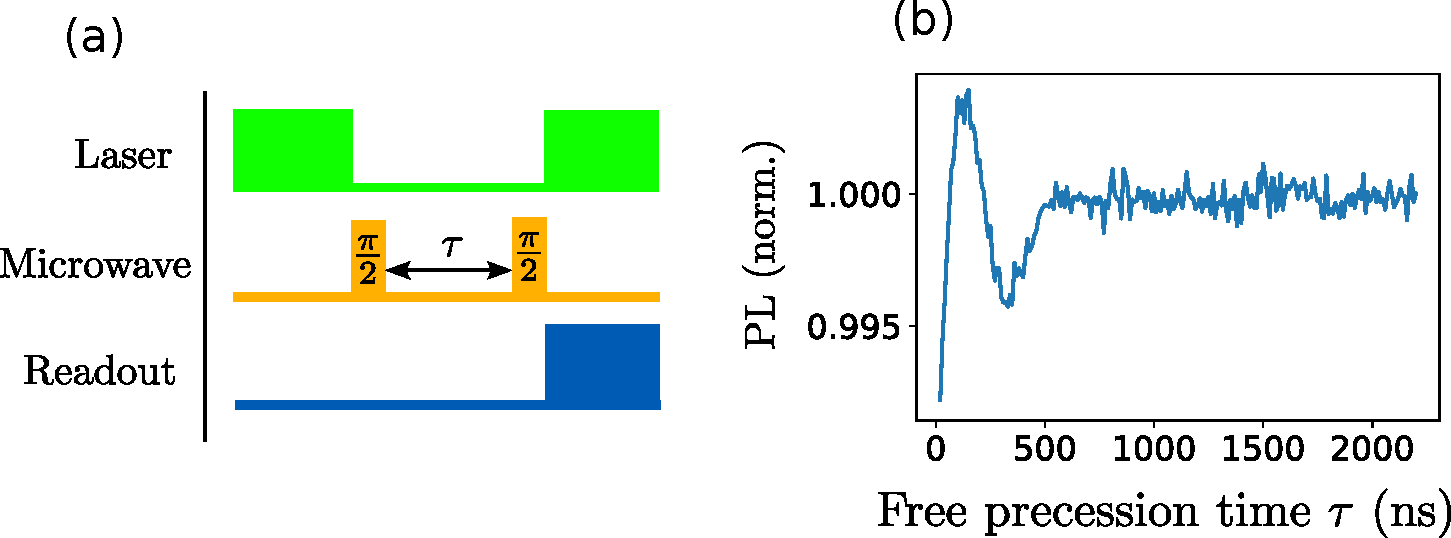
\includegraphics[width=\textwidth]{Figures/Ramsey}
\caption{Ramsey interferometry protocol. (a) Pulse seqeunce used. (b) Experimental data obtained on sample CVD-pink.} %The orange line corresponds to an Gaussian fit with time constant $\tau=400 \pm 100\ \rm ns$.}
\label{Ramsey}
\end{figure}

The $T_2^*$ time is the characteristic time for the loss of quantum coherence of a freely evolving system. It is generally defined as the decay time of of a Ramsey interferometry measurement \citep{barry2020sensitivity}.

Fig. \ref{Ramsey} shows the Ramsey pulse sequence and an  example obtained on a spin ensemble. The microwave frequency is detuned by $\sim 300\ \rm kHz$ compared to the spin central Larmor frequency which causes oscillations in the signal. $T_2^*$ is the decay time of the envelope of the Ramsey fringes. Unfortunately, it is hard to correctly fit the envelope of a signal with so few fringes. Increasing the number of fringes with our current microwave and optical setup might prove hard, as further microwave detuning would decrease the signal contrast, and would be ultimately limited by the microwave pulses resolution.

Ramsey sequences are generally harder to perform on NV ensemble than they are on single NV for two main reasons. The first one is that the $T_2^*$ times tend to be longer for single NV centers as they do not suffer from spatial inhomogeneity, and because the samples used for single NV experiments generally contains less impurities than those used for NV ensemble. The second one is the inhomogeneous microwave power which leads to a variation of the Rabi frequencies among the spins \citep{barry2016optical, zhou2020quantum} and lowers the fringe contrast.

An alternative measurement of $T_2^*$ can be performed by looking at the linewidth of an ODMR spectrum. Indeed, ideally the ODMR spectrum should be the Fourier transform of the Ramsey signal (also called free induction decay in NMR literature). In practice however, both methods suffer from experimental noises and imperfections, with Ramsey-type methods being more sensitive to microwave inhomogeneities \citep{barry2020sensitivity} while ODMR is prone to laser and microwave power broadening \citep{dreau2011avoiding}. 

The method chosen to extract $T_2^*$ values in this manuscript was ODMR with low microwave power ($\Omega_{\rm Rabi} \ll 1/T_2^*$) and low laser intensity (compared to the the NV optical saturation).

\subsubsection{Physical origin}

\begin{figure}[h!]
\centering
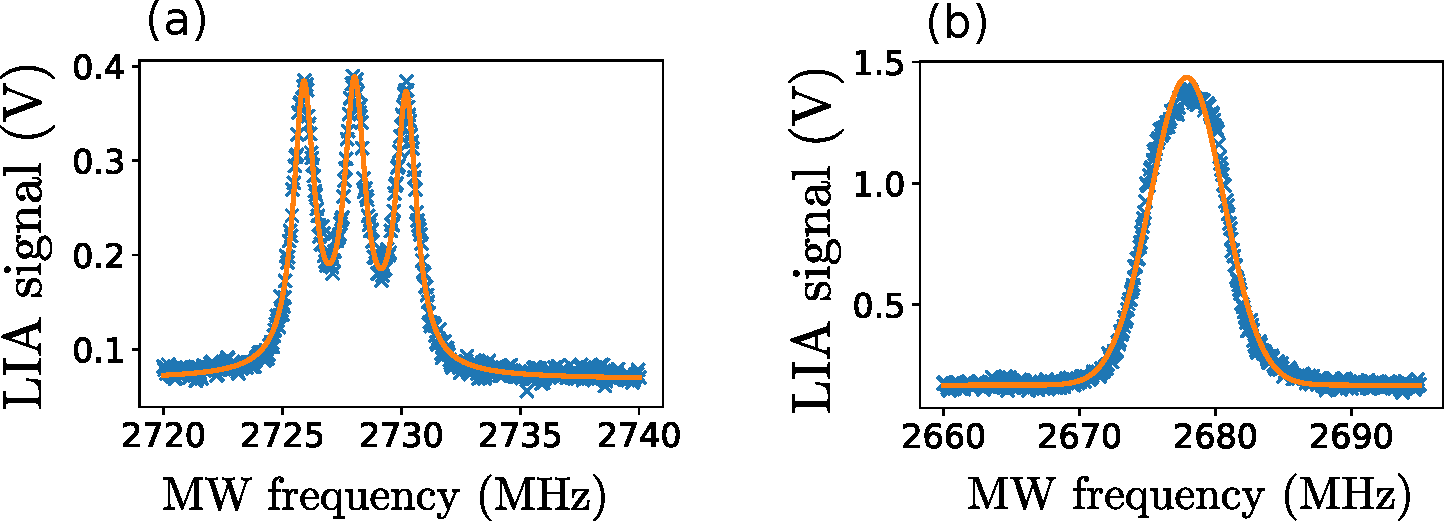
\includegraphics[width=\textwidth]{Figures/ODMR_1_classes}
\caption{ODMR spectra on a single NV class. (a) Experimental data on sample CVD-pink, fitted with three Lorentzians with HWHM $530$ kHz ($T_2^*=300\ \rm ns$). (b) Experimental data on sample Sumi-2, fitted with a single Gaussian with HWHM $3.2$ MHz ($T_2^*=83 ns$).}
\label{ODMR 1 classe}
\end{figure}

For most samples, the leading cause of inhomogeneous dephasing is the temporal and spatial variations of magnetic fields caused by the paramagnetic impurities in the crystal \citep{barry2020sensitivity}. The nature of these different paramagnetic impurities will be further discussed in the section dedicated to dark spins in diamond in chapter 2. We will simply mention here that for sample with high NV density ([NV] $\geq$ ppm), $T_2^*$ is mostly limited by the electronic spins of nitrogen impurities \citep{bauch2018ultralong}.

Fig. \ref{ODMR 1 classe} shows ODMR spectra of a single NV class on two distinct samples (see [REF]). The first sample is a CVD sample with a total substitutional nitrogen  concentration $[N_s] \approx 26\ \rm ppm$, while the second is a type-Ib HPHT sample with a likely nitrogen concentration $[N_s] \geq 100\ \rm ppm$. We can clearly see a higher linewidth, corresponding to a smaller $T_2^*$ value on the sample with higher nitrogen concentration. In particular, we can notice the hyperfine structure of the $^{14}$N nuclei on the CVD sample, whereas it is hidden by the inhomogeneous broadening on the HPHT sample.

Fig. \ref{ODMR 1 classe} illustrates another difficulty of $T_2^*$ measurement which is to find the correct fitting formula. While the spectral profile of single NV centers is expected to be Gaussian, the spectral profile of an ensemble of NV centers  is expected to be Lorentzian \citep{dobrovitski2008decoherence, hall2014analytic}. For Fig. \ref{ODMR 1 classe}-a), it was indeed found that Lorentzians fitted the data better than Gaussians. For Fig. \ref{ODMR 1 classe}-b) however, a Gaussian was found to be a better fit than a Lorentzian, although this could be in part due to the unresolved hyperfine structure.

\subsection{NV spin $T_2$}
\begin{figure}[h!]
\centering
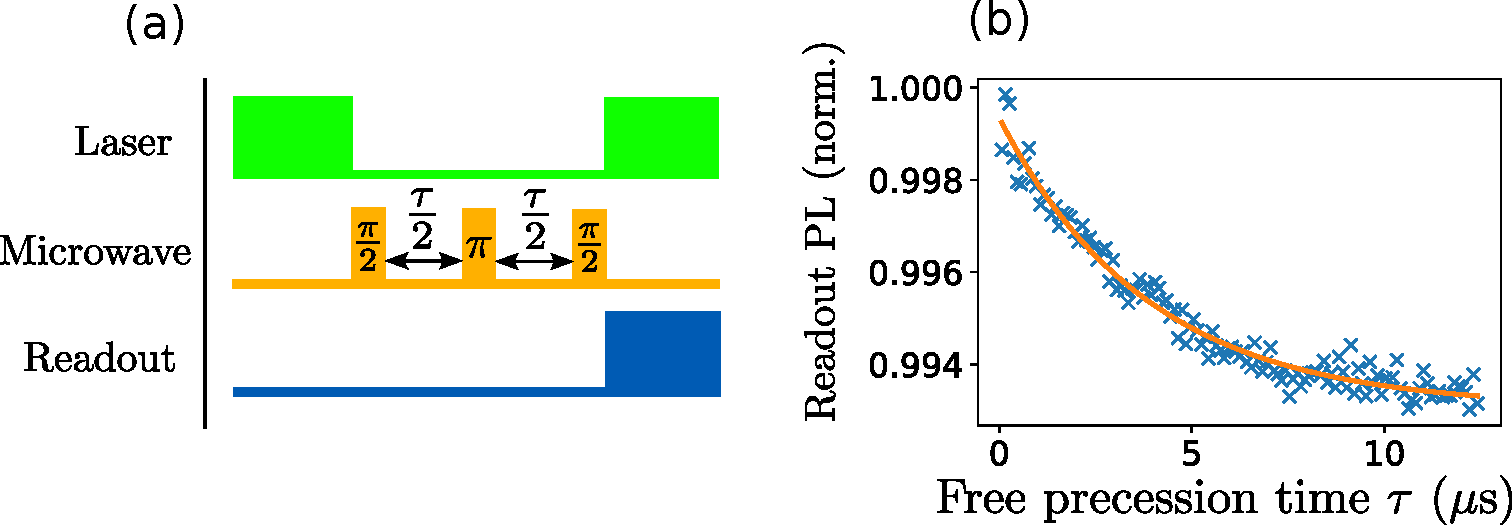
\includegraphics[width=\textwidth]{Figures/Echo}
\caption{Spin-echo protocol. (a) Pulse seqeunce used. (b) Experimental data obtained on sample CVD-pink, fitted with an exponential decay of time $3.9\ \rm{\mu s}$.} 
\label{Echo}
\end{figure}
\subsubsection{Measurement protocol}
As precised earlier, the exact $T_2$ definition depends on the rephasing scheme used. We will focus here on the simplest known rephasing process which is the spin-echo or Hahn-echo sequence.

Fig. \ref{Echo} shows the pulse sequence used and an example on the same sample than the Ramsey measurement. The pulse sequence differs from the Ramsey one by adding a a $\pi$-pulse in the middle of the free precession time. This additional $\pi$-pulse causes static or slowly varying dephasing to be rephased \citep{hahn1950spin}. 

This protocol extends the coherence time on this particular sample from $T_2^* \approx 300\ \rm ns$ to $T_2 \approx 4\ \rm{\mu s}$, an increase by more than a factor of 10. Improvement by a factor of $10 \sim 100$ or typical for NV ensembles \citep{barry2020sensitivity}. This value could likely be extended even further by using a more complex dynamical decoupling scheme from the CPMG or XY sequence families \citep{naydenov2011dynamical, bar2012suppression}.

\subsubsection{Physical origin}
The origin of the relaxation time $T_2$ are fluctuating noises which are too fast to be efficiently rephased by the sequence. The origin of these noises is generally attributed to the flipping of spins in the vicinity of the NV center (either through spin-lattice or spin-spin mechanisms) \citep{hall2014analytic}. For samples with high nitrogen concentration, it has been measured that the $T_2$ time  was directly correlated to the nitrogen concentration, with the same scaling than the $T_2^*$ time \citep{bauch2019decoherence}.

\section{Dipole-dipole interaction between two electronic spins}

\begin{figure}[h!]
\centering
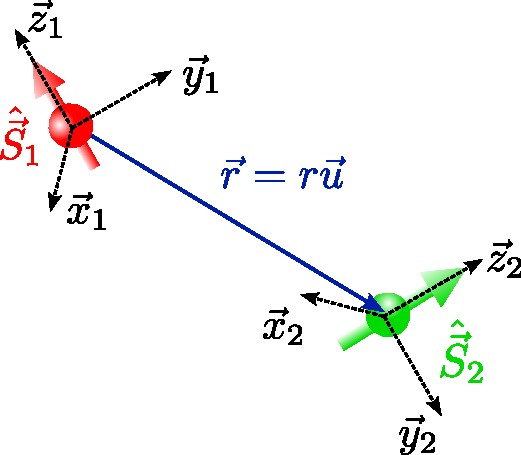
\includegraphics[width=0.4\textwidth]{Figures/shema_dipole_dipole}
\caption{Geometric representation of two interacting spins. ($\mathbf{x}_1,\mathbf{y}_1,\mathbf{z}_1$) and ($\mathbf{x}_2,\mathbf{y}_2,\mathbf{z}_2$) represent Cartesian coordinate systems in the spin frames of reference, where $\mathbf{z}_i$ is the axis of quantization of spin $i$.} 
\label{dipole-dipole}
\end{figure}

This final introductory section will focus on the dipole-dipole interaction between two electronic spins, which is the main form of spin-spin interaction and plays a key part in the properties of dense spin ensemble. 

We will consider the general situation represented in Fig. \ref{dipole-dipole}: two spins separated by a distance $r$ with their own coordinate systems ($\mathbf{x}_1,\mathbf{y}_1,\mathbf{z}_1$) and ($\mathbf{x}_2,\mathbf{y}_2,\mathbf{z}_2$). The coordinate system is chosen so that each spin operator can be written:

\begin{equation}
\hat{\mathbf{S}}_i=\hat{S}_x \mathbf{x}_i + \hat{S}_y \mathbf{y}_i + \hat{S}_z \mathbf{z}_i
\end{equation}

where the spin operators $\hat S_{\{x,y,z\} }$ have their usual definitions in term of Pauli matrices. In particular, this means that the spin axis of quantization of each spin is $z_i$, which classically corresponds to the magnetization direction of the dipole. This axis can be defined either by the magnetic field, or by crystal field anisotropies, as is often the case for solid state spins with $S\geq 1$ (including the NV center).

\subsection{Magnetic dipole-dipole Hamiltonian}

Classically, the dipole-dipole interaction between two magnetic moments $\mathbf{m}_1$ and $\mathbf{m}_2$ can be derived by computing the static magnetic field generated by one dipole at the position of the second dipole \cite[p.~188]{jackson1999classical}:

\begin{align}
U&=-\mathbf{m}_1 \cdot \mathbf{B}(\mathbf{r}) \nonumber \\
&=-\frac{\mu_0}{4 \pi}\left[ \frac{3 (\mathbf{m}_1\cdot\mathbf{u})(\mathbf{m}_2\cdot\mathbf{u}) - \mathbf{m}_1\cdot\mathbf{m}_2}{r^3}+\frac{8\pi}{3}\mathbf{m}_1\cdot\mathbf{m}_2\,\delta(r)\right], \label{eq. dipole classique}
\end{align}

where $\mathbf{r}=r \mathbf{u}$ is the relative position of the two dipoles (see Fig. \ref{dipole-dipole}). 

The quantum analog of the dipole-dipole interaction between spins simply replaces the magnetic moments $\mathbf{m}_i$ in eq. (\ref{eq. dipole classique}) with $\hbar \gamma_i \hat{\mathbf{S}}_i$, where $\gamma_i$ is the gryromagnetic ratio and $\hat{\mathbf{S}}_i$ the spin vector operator for spin $i$:

\begin{equation}
\mathcal{H}_{\rm dd}=\frac{\mu_0 \gamma_1 \gamma_2 \hbar^2}{4 \pi}\left[ \frac{3 (\hat{\mathbf{S}}_1\cdot\mathbf{u})(\hat{\mathbf{S}}_2\cdot\mathbf{u}) - \hat{\mathbf{S}}_1\cdot\hat{\mathbf{S}}_2}{r^3}+\frac{8\pi}{3}\hat{\mathbf{S}}_1\cdot\hat{\mathbf{S}}_2\,\delta(r)\right].
\end{equation}

The $\delta(r)$ term represents the Fermi contact energy. This term plays an important role when there is an overlap of the spin particle wavefunctions, such as the hyperfine coupling between the NV$^-$ electron spin and $^{14}$N \cite{doherty2012theory} or  $^{13}$C \cite{smeltzer201113c} nuclear spins.

The focus of this manuscript is on the interaction between electronic spins which are separated by several atomic sites (density impurities in the $\sim$ ppm range). We will therefore assume that there is negligible overlap between the electronic wavefunctions and omit the Fermi contact term. This leads the simplified dipole-dipole Hamiltonian:

\begin{equation}
\mathcal{H}_{\rm dd}= \frac{J_0}{r^3}\left[ 3 (\hat{\mathbf{S}}_1\cdot\mathbf{u})(\hat{\mathbf{S}}_2\cdot\mathbf{u}) - \hat{\mathbf{S}}_1\cdot\hat{\mathbf{S}}_2] \right],
\end{equation}

where $J_0=\frac{\mu_0 \gamma_1 \gamma_2 \hbar^2}{4 \pi}$.

For two electronic spins with $g$-factors $\approx -2$\footnote{Most spin defects in diamond, including the NV center have a g-factor $\approx -2$ similarly to free electrons.}, 
\begin{equation*}
\frac{J_0}{h} \approx 51.8\ \rm{MHz}\cdot \rm{nm}^3.
\end{equation*}

\subsection{Decomposition of the dipole-dipole Hamiltonian}

\begin{figure}[h!]
\centering
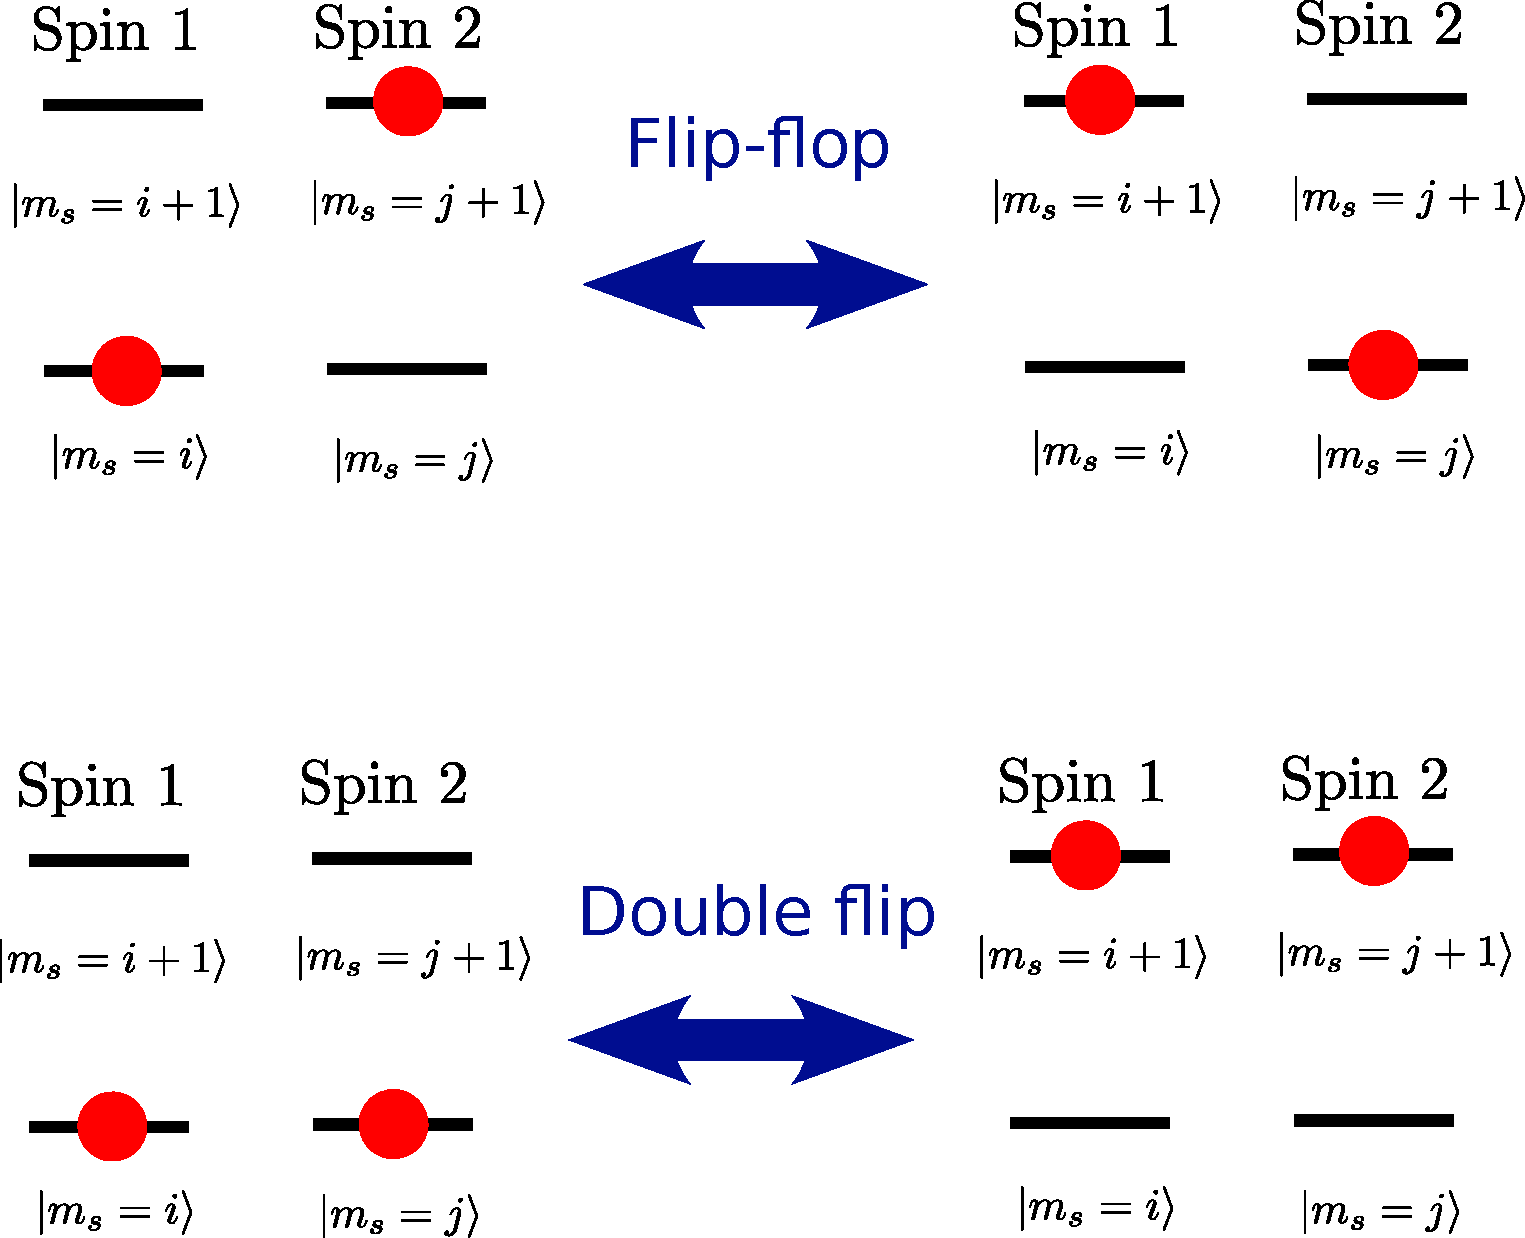
\includegraphics[width=.7\textwidth]{Figures/flip-flop_double-flip}
\caption{Representation of the two energy transfer mechanisms: flip-flop and double flips} 
\label{flip flop double flip}
\end{figure}

In the weak coupling approximation, the dipole-dipole Hamiltonian between two spins can be decomposed between diagonal terms which are responsible for energy shifts of the individual spin levels, and the off-diagonal terms which are responsible for energy transfers between the two spins.

In what follows, we will assume that both spins have the same quantization axis in order to simplify the Hamiltonian decomposition. A more general case is detailed in [REF].

Following the notation introduced in Fig. \ref{dipole-dipole}, we will then assume that $$(\mathbf{x}_1,\mathbf{y}_1,\mathbf{z}_1) = (\mathbf{x}_2,\mathbf{y}_2,\mathbf{z}_2) = (\mathbf{x},\mathbf{y},\mathbf{z}).$$ We will denote $\mathbf{u}=u_x \mathbf{x} + u_y \mathbf{y} + u_z \mathbf{z}$ the decomposition of the unitary vector $\mathbf{u}$ in this basis. The dipole-dipole Hamiltonian can then be written:
\begin{equation}
\mathcal{H}_{\rm dd}=\frac{J_0}{r^3}\left[ (3 u_x^2-1) S_x^1 S_x^2 + (3 u_y^2-1) S_y^1 S_y^2 + (3 u_z^2-1) S_z^1 S_z^2 \right],
\end{equation}
where $S_{\{x,y,z\} }^i$ are the spin operators acting on spin $i$. The $S_z^1 S_z^2$ term is the only diagonal term and corresponds to energy shifts while the $S_x^1 S_x^2$ and $S_y^1 S_y^2$ terms are responsible for energy transfer. To make the transfer mechanism more apparent, we will rewrite $S_x^i$ as $\frac{1}{2}(S_+^i+S_-^i)$ and $S_y^i$ as $\frac{1}{2i}(S_+^i-S_-^i)$:
\begin{align}
\mathcal{H}_{\rm dd}&=\frac{J_0}{r^3}\bigg{[} \frac{1}{4}(3 u_x^2 + 3 u_y^2 -2)(S_+^1 S_-^2 + S_-^1 S_+^2) \nonumber \\
&\quad + \frac{1}{4}(3 u_x^2 - 3 u_y^2)(S_+^1 S_+^2 + S_-^1 S_-^2) \nonumber \\
&\quad +(3 u_z^2-1) S_z^1 S_z^2 \bigg{]} \nonumber \\
\medskip
&= \Omega_{\rm ff} (S_+^1 S_-^2 + S_-^1 S_+^2) + \Omega_{\rm df} (S_+^1 S_+^2 + S_-^1 S_-^2) + \Omega_{\rm shift} S_z^1 S_z^2. \label{eq. ff df}
\end{align}

We have introduced in eq. (\ref{eq. ff df}) the three relevant matrix elements $\Omega_{\rm ff}$, $\Omega_{\rm df}$, and $\Omega_{\rm shift}$ which correspond respectively to flip-flops, double flips and energy shifts. Flip-flops and double flips (sometimes referred as flip-flips) are represented in Fig. \ref{flip flop double flip}. Flip flops correspond to energy transfer between two spins for which the sum of the spin angular momentum is conserved ($\Delta (m_s^1+m_s^2)=0$), while double flips correspond to energy transfer for which the spin angular momentum is not conserved ($\Delta (m_s^1+m_s^2)=\pm 2$)\footnote{In order to preserve the total angular momentum, double flips transfer angular moment to the crystal, which is a form of Einstein de Haas effect \citep{einstein1915experimental} }. In both cases however, the energy between the initial and final states needs to be preserved for the transfer to be efficient. 

It should be noted that on average, each matrix element is of the same order of magnitude: $\Omega_{\rm ff} \sim \Omega_{\rm df} \sim \Omega_{\rm shift} \sim \frac{J_0}{r^3}$. 

\subsection{Cross-relaxations with NV centers}

\begin{figure}[h]
\centering
\includegraphics[width=0.9\textwidth]{Figures/Shema_CR}
\caption{Illustration of cross-relaxations between an NV center and an unpolarized spin. Red dots represent the population in each states, and the arrows the various population transfer mechanisms}
\label{CR_shema}
\end{figure}

Cross-relaxation (CR) is the transfer of polarization from one spin to another (or more generally from one family of spins to another family). This process can occur through either flip-flops or double flips, as long as the resonance condition between the two spins is met. 

On of the condition for cross-relaxation is to have a difference in polarization between the two spins species considered. The NV center is therefore a good candidate to observe cross-relaxations as it can be optically polarized while most other spin species are not. 

Fig. \ref{CR_shema} illustrates CR between a polarized NV center and an unpolarized second spin. When the two considered spin transitions become resonant, in this case by tuning the magnetic field, polarization from the NV center will be transferred to the second spin, making the NV center less polarized and the second spin more polarized than when they are out of resonance. 

For a single NV center coupled to spin 2, assuming that spin 2 always remains depolarized\footnote{This is the case in practice if the spin 2 bath is much bigger than the NV bath and effectively acts as a thermostat, or if the lifetime of spin 2 is much smaller than that of the NV center.} and that the coupling strength between the two spins is smaller than their respective dephasing time $T_2^*$ (weak coupling regime), the modification in the NV relaxation rate $\Gamma_1=\frac{1}{T_1}$ caused by the cross-relaxation with spin 2 can be analytically computed \citep{hall2016detection}:
\begin{equation}
\delta \Gamma_1=\frac{\Omega^2}{\Gamma_2^*} \frac{(\Gamma_2^*)^2}{(\delta \nu)^2+(\Gamma_2^*)^2},
\label{delta gamma 1}
\end{equation}
where $\Gamma_2^*=\frac{1}{T_2^*(\rm NV)}+\frac{1}{T_2^*(\rm Spin 2)}$ is the joint dephasing rate of the NV center and the second spin, $\delta \nu$ is the detuning in energy (expressed in frequency) between the initial and final states and $\Omega=\Omega_{\rm ff}$ or $\Omega_{\rm df}$ is the dipole-dipole matrix element corresponding to the flip-flop or double-flip process considered. 

Eq. (\ref{delta gamma 1}) is the basis for every cross-relaxation detection performed in this manuscript. Because the NV center lifetime can be measured optically, as detailed in Sec. \ref{sec T1 NV}, cross-relaxation between NV-centers and other spin species can be measured optically. Measuring the cross-relaxation depolarization can then be used to gain information on the second spin or on the dipole-dipole interaction mechanisms, as will be explained in the following chapters.

\section{Conclusion}

We have covered in this introductory chapter every concepts needed to understand the results presented in the next chapters. We have seen the main steps in the creation of artificial diamonds and NV centers, we have covered the optical and spin properties of the NV center as well as the ways to measure them, and we have introduced the notion of dipole-dipole coupling and cross-relaxation between two spins.

The focus of chapter 2 will be on the cross-relaxation between NV centers and other spin impurities in CVD-grown diamond, while the focus of chapter 3 and 4 will be on the cross-relaxation between NV centers and other NV centers, as well as their potential application in magnetometry.
\printbibliography
\end{document}
